% ===================================================================
%  Spinal Cord qMRI Harmonization — LaTeX Manuscript
%  Target journals: Scientific Reports / Frontiers in Neurology /
%                   BMC Medical Imaging / NeuroImage
% ===================================================================
\documentclass[12pt,a4paper]{article}

% ---- Packages ----
\usepackage[utf8]{inputenc}
\usepackage[T1]{fontenc}
\usepackage{amsmath,amssymb}
\usepackage{graphicx}
\usepackage{booktabs}
\usepackage[margin=2.5cm]{geometry}
\usepackage{hyperref}
\usepackage{setspace}
\usepackage{caption}
\usepackage{subcaption}
\usepackage{enumitem}
\usepackage{natbib}
\usepackage{xcolor}
\usepackage{float}
\usepackage{lineno}
\usepackage{authblk}
\usepackage{multirow}

\hypersetup{
    colorlinks=true,
    linkcolor=blue,
    citecolor=blue,
    urlcolor=blue
}

\onehalfspacing

% ---- Title & Authors ----
\title{\textbf{Impact of Scanner Vendor Harmonization on Spinal Cord Quantitative MRI Biomarkers:\\
A Systematic Benchmark of Five Statistical Correction Strategies}}

\author[1]{Yilin Zhu}
\author[2,*]{Dengke Wu}

\affil[1]{Changsha Hospital of Traditional Chinese Medicine (Changsha No.~8 Hospital), Changsha City, Hunan Province, China}
\affil[2]{Department of Emergency Medicine, and Emergency Medicine and Difficult Diseases Institute, The Second Xiangya Hospital of Central South University, Changsha 410011, Hunan, China}

\date{}

% Corresponding author marker
\newcommand{\corresponding}[1]{\thanks{Corresponding author: #1}}

\begin{document}
\linenumbers

\maketitle

\renewcommand{\thefootnote}{\fnsymbol{footnote}}
\footnotetext[0]{Corresponding author: Dengke Wu, Department of Emergency Medicine, and Emergency Medicine and Difficult Diseases Institute, The Second Xiangya Hospital of Central South University, Changsha 410011, Hunan, China. Email: \texttt{wudk2010@csu.edu.cn}}
\renewcommand{\thefootnote}{\arabic{footnote}}
\setcounter{footnote}{0}

% ===================================================================
\section*{Abstract}

Quantitative spinal cord MRI biomarkers exhibit systematic vendor-dependent variability that limits multi-center pooling. Although harmonization methods developed for brain imaging are increasingly adopted, a systematic spinal cord benchmark---jointly evaluating vendor-effect removal, biological-signal recovery, and subject-level preservation---is absent. Eight qMRI biomarkers across four families (T2w, T2*, MT, DTI) were extracted at C2--C3 from the spine-generic multi-subject dataset (267 subjects, 44 sites, 3 vendors). Five methods---per-metric ComBat, ComBat-joint, CovBat, RELIEF, and LME/FE---were evaluated on three endpoints: residual vendor effect ($\eta^2$, ICC, PERMANOVA $R^2$), biological-signal recovery (age/sex semi-partial $R^2$), and subject-level preservation (pre-post Pearson $r$) in HC ($N=188$) and pathology-inclusive ($N=246$) cohorts. Baseline vendor effects were large ($\eta^2 = 0.28$; PERMANOVA $R^2 = 0.32$, $p < 10^{-4}$), exceeding age-related variance by $\sim$two orders of magnitude and sex-related variance by $\sim$one order of magnitude. All methods reduced vendor $\eta^2$ by $>99.8\%$, rendering multivariate vendor structure non-significant (all $p \geq 0.97$). Age signal increased 2.3--3.7-fold. Methods diverged on subject preservation: LME/FE highest ($r = 0.84$), CovBat lowest ($r = 0.78$), forming a Pareto frontier. Harmonization is recommended for pooled multi-vendor spinal cord qMRI; method choice should match the downstream analytic goal---LME/FE or ComBat for subject-level inference, CovBat/RELIEF for pooled-group analyses.

\vspace{4mm}
\noindent\textbf{Keywords:} spinal cord MRI $\cdot$ quantitative imaging $\cdot$ multi-center harmonization $\cdot$ ComBat $\cdot$ PERMANOVA $\cdot$ biomarker reproducibility

\noindent\textbf{Abbreviations:} ComBat = Combatting batch effects; CovBat = Covariance Batch harmonization; LME/FE = linear mixed-effects / fixed-effects hybrid model (see \S~2.3); RELIEF = Removal of Latent Inter-scanner Effects via independent components; PERMANOVA = permutational multivariate analysis of variance; ICC = intraclass correlation coefficient; CSA = cross-sectional area; MTR = magnetization transfer ratio; MTsat = magnetization transfer saturation; FA = fractional anisotropy; MD/AD/RD = mean/axial/radial diffusivity; EB = empirical Bayes; HC = healthy control; DCM = degenerative cervical myelopathy.

\newpage

% ===================================================================
\section{Introduction}

Quantitative magnetic resonance imaging (qMRI) of the spinal cord has emerged as a cornerstone for characterizing neurological disease progression and treatment response. Cross-sectional area (CSA), magnetization transfer ratio (MTR), magnetization transfer saturation (MTsat), and diffusion tensor metrics (FA, MD, AD, RD) are now routinely included in multi-center spinal cord protocols \cite{cohen2021opena} and provide non-invasive windows into cord atrophy, demyelination, and axonal integrity in multiple sclerosis, degenerative cervical myelopathy (DCM), spinal cord injury, and amyotrophic lateral sclerosis \cite{freund2024dcm}.

A central obstacle to translating these biomarkers from single-center research to large-scale clinical and epidemiological applications is their measurable, non-biological variability across MRI vendors. Even when standardized acquisition protocols are followed---as in the spine-generic consensus protocol \cite{cohen2021opena,cohen2021generic}---differences in gradient hardware, RF coil geometry, vendor-specific reconstruction pipelines, and intrinsic sequence implementations introduce systematic offsets and scale changes in derived biomarkers. The magnitude of these vendor effects is often comparable to---or larger than---the biological effect sizes of interest, biasing group comparisons and inflating between-site variance in longitudinal pooling. This problem is particularly acute in spinal cord imaging: the cord's small cross-section (typically 60--90~mm$^2$) relative to voxel dimensions magnifies partial-volume effects, motion artifacts, and CSF pulsation, creating a noise floor that interacts non-trivially with batch-effect estimators \cite{prados2017spinal}.

Statistical post-hoc harmonization---correcting derived biomarker values rather than re-acquiring images---has emerged as a tractable, scalable solution. The foundational method, ComBat \cite{johnson2007adjusting,fortin2017harmonization}, models site as a location-and-scale shift with empirical Bayes (EB) shrinkage of site-specific parameters. Extensions include CovBat \cite{chen2022mitigating}, which additionally harmonizes cross-feature covariance via principal-component correction, and RELIEF \cite{zhang2023relief}, which uses independent component analysis (ICA) to identify and remove batch-loaded latent factors while preserving orthogonal biological variation. A simpler alternative---a linear mixed-effects (LME) model with site/vendor as a random intercept---adjusts for mean shifts while preserving per-subject deviations.

While these methods have been benchmarked extensively in brain imaging \cite{fortin2018harmonization,tax2019cross,bayer2022site}, their performance on spinal cord biomarkers remains uncharacterized. Middleton et al.\ recently demonstrated that ComBat harmonization substantially improves inter-scanner agreement for cervical and thoracic spinal cord DTI metrics \cite{middleton2023spinal}, and Jodoin et al.\ provided best-practice guidance for ComBat deployment in diffusion MRI \cite{jodoin2025combat}. However, no study has systematically compared the full ComBat family (including CovBat and RELIEF) across a comprehensive panel of spinal cord qMRI biomarkers using unified, multi-endpoint evaluation \cite{destefano2022magnims}. Three considerations make the spinal cord a distinct and demanding harmonization target: (i) the smaller per-site sample sizes typical of spinal cord consortia (often 5--15 subjects per site) challenge EB shrinkage reliability; (ii) the strong inter-metric correlation among spinal cord biomarkers (e.g., diffusion metrics are intrinsically coupled; MTR and MTsat share acquisition-dependent variance) motivates evaluation of multivariate---not merely univariate---decontamination; and (iii) the clinical need to preserve disease-related variance while removing site effects creates a tension that no existing benchmark has systematically quantified.

The spine-generic multi-subject dataset \cite{cohen2021opena,cohen2021generic} has been used to establish normative spinal cord morphometry references \cite{valosek2024morphometry}, characterize longitudinal qMRI reproducibility \cite{boudreau2025longitudinal}, and validate contrast-agnostic segmentation algorithms \cite{bedard2025contrast}, but has not been used to benchmark post-hoc statistical harmonization strategies for cross-vendor biomarker pooling. Here we present a systematic comparison of five statistical harmonization methods applied to eight standard spinal cord qMRI biomarkers extracted from this dataset. For each method we quantify three orthogonal endpoints: (i) residual vendor effect (univariate $\eta^2$, ICC, and multivariate PERMANOVA $R^2$); (ii) recovery of biological signal (age and sex semi-partial $R^2$); and (iii) preservation of within-vendor subject-level ranking (Pearson $r$ between pre- and post-harmonization values). We report results in both a healthy-control cohort (HC, $N=188$) that isolates pure vendor-driven variance, and a pathology-inclusive cohort (ALL, $N=246$) that approximates real-world deployment.

This study extends prior spinal cord harmonization work in four respects that collectively address the gap between the brain-imaging benchmark literature and practice in the spinal cord. First, whereas Middleton et al.\ \cite{middleton2023spinal} demonstrated ComBat's effectiveness for spinal cord DTI metrics on a per-metric basis, we formally compare the \emph{full ComBat family}---including the more aggressive covariance (CovBat) and latent-factor (RELIEF) extensions whose multivariate behavior is unknown for spinal cord data---across a comprehensive panel of eight biomarkers spanning four acquisition families (T2w, T2*, MT, DTI). This enables direct assessment of whether the additional variance components modeled by CovBat and RELIEF confer meaningful benefit over standard ComBat in the spinal cord context. Second, we introduce a three-axis evaluation framework that jointly quantifies vendor removal, biological-signal preservation, and subject-level ranking---whereas existing spinal cord studies have evaluated only one or two of these dimensions simultaneously. Third, we employ PERMANOVA as a multivariate endpoint, which captures residual vendor-specific covariance patterns that univariate $\eta^2$ or ICC alone can miss. Fourth, we formalize the observed trade-off between multivariate decontamination and subject-level preservation as a Pareto frontier, providing an actionable, transparent decision rule for method selection. Our central finding is that methods occupy a reproducible Pareto frontier in the trade-off between multivariate vendor decontamination and subject-level preservation---a result that provides quantitative, actionable guidance for method selection in multi-center spinal cord studies.

% ===================================================================
\section{Materials and Methods}

\subsection{Dataset and Cohort Definition}

All analyses used the openly distributed \emph{spine-generic multi-subject dataset} (release r20240523) \cite{cohen2021opena}, comprising 267 subjects scanned at 44 sites on 13 distinct scanner models from three vendors (GE Healthcare: 37 subjects; Philips: 50 subjects; Siemens Healthineers: 180 subjects) using the standardized spine-generic consensus protocol. The dataset is BIDS-compliant and includes T1-, T2-, and T2*-weighted structural images, magnetization-transfer-weighted images for MTR/MTsat computation, and a diffusion-weighted sequence at the cervical level. Demographic covariates---age, sex, height, and weight---were balanced across vendors (ANOVA/$\chi^2$: age $p = 0.125$, sex $p = 0.643$, height $p = 0.232$, weight $p = 0.576$; Table~1), ruling out demographic confounding as an explanation for observed vendor effects.

\textbf{Cohort flow.} Of the 267 subjects, 203 were healthy controls (HC) and 64 had pathology (62 mild cervical compression; 2 DCM). Twenty-one subjects (15 HC, 6 pathology) were missing one or more biomarkers---primarily MTR ($n=13$ missing) and MTsat ($n=18$ missing), with diffusion metrics missing for 7 subjects each---yielding 188 HC and 246 ALL complete-case subjects. Missingness was determined by acquisition failure or quality-control rejection during pipeline processing (automated SCT QC metrics including segmentation overlap with PAM50 template, diffusion tensor model fit residual, and MT saturation map artifact screening, as specified in the spine-generic processing pipeline documentation; \url{https://spine-generic.readthedocs.io}), not by demographic or vendor characteristics, ruling out informative missingness.

Two cohorts were defined prior to analysis:
\begin{itemize}[nosep]
  \item \textbf{HC cohort} ($N=203$ with $\geq 1$ complete biomarker; $N=188$ complete on all eight metrics): healthy controls only. This cohort isolates vendor-driven variance from any pathological signal and constitutes the conservative reference for evaluating harmonization specificity.
  \item \textbf{ALL cohort} ($N=267$ with $\geq 1$ complete biomarker; $N=246$ complete on all eight metrics): healthy controls together with participants with mild cervical compression and DCM. This cohort approximates real-world deployment where harmonization must remove vendor effects without erasing disease-related variance. Pathology distribution was balanced across vendors ($\chi^2$ $p = 0.661$).
\end{itemize}

\begin{table}[H]
\centering
\caption{Demographic and acquisition characteristics by vendor (HC cohort, all subjects $N=203$; complete-case subset $N=188$ used for joint-method analyses).}
\label{tab:demographics}
\begin{tabular}{lccccr}
\toprule
\textbf{Characteristic} & \textbf{GE ($n=28$)} & \textbf{Philips ($n=36$)} & \textbf{Siemens ($n=139$)} & \textbf{Total ($n=203$)} & \textbf{$p$-value} \\
\midrule
Age (years)       & 26.9 $\pm$ 4.7 & 28.2 $\pm$ 4.5 & 29.1 $\pm$ 5.9 & 28.7 $\pm$ 5.6  & 0.125 \\
Sex (\% female)    & 53.6           & 52.8           & 46.0           & 48.3             & 0.643 \\
Height (cm)        & 169.6 $\pm$ 8.5 & 172.2 $\pm$ 10.2 & 173.2 $\pm$ 10.0 & 172.5 $\pm$ 9.9  & 0.232 \\
Weight (kg)        & 65.2 $\pm$ 13.7 & 67.6 $\pm$ 14.3 & 68.2 $\pm$ 13.1 & 67.7 $\pm$ 13.4  & 0.576 \\
Scanner models     & 3              & 4              & 6              & 13               & --- \\
\bottomrule
\end{tabular}
\vspace{4pt}
\par\small\textit{Note:} Continuous variables: mean $\pm$ SD, one-way ANOVA across vendors. Categorical: $\chi^2$ test. The demographic balance across vendors is a critical precondition---any vendor effects observed in biomarkers cannot be attributed to confounding by age, sex, or body habitus. For the ALL cohort ($N=246$), pathology distribution (HC / mild compression / DCM) was also balanced across vendors ($\chi^2$ $p = 0.661$); see Table~\ref{tab:demographics_all} for ALL-cohort demographics.
\end{table}

\begin{table}[H]
\centering
\caption{Demographic and acquisition characteristics by vendor (ALL cohort, $N=246$).}
\label{tab:demographics_all}
\begin{tabular}{lccccr}
\toprule
\textbf{Characteristic} & \textbf{GE ($n=33$)} & \textbf{Philips ($n=47$)} & \textbf{Siemens ($n=166$)} & \textbf{Total ($n=246$)} & \textbf{$p$-value} \\
\midrule
Age (years)       & 28.0 $\pm$ 5.2 & 29.4 $\pm$ 4.7 & 30.0 $\pm$ 6.3 & 29.6 $\pm$ 5.9  & 0.193 \\
Sex (\% female)    & 48.5           & 46.8           & 47.0           & 47.2             & 0.986 \\
Height (cm)        & 169.2 $\pm$ 8.5 & 171.5 $\pm$ 10.2 & 172.8 $\pm$ 10.2 & 172.3 $\pm$ 10.0  & 0.182 \\
Weight (kg)        & 66.4 $\pm$ 12.7 & 68.0 $\pm$ 15.5 & 68.3 $\pm$ 12.9 & 68.0 $\pm$ 13.3  & 0.767 \\
Pathology (HC/MC/DCM) & 25/8/0 & 33/13/1 & 130/35/1 & 188/56/2 & 0.661 \\
Scanner models     & 3              & 4              & 6              & 13               & --- \\
\bottomrule
\end{tabular}
\vspace{4pt}
\par\small\textit{Note:} MC = mild cervical compression; DCM = degenerative cervical myelopathy. Pathology distribution balanced across vendors ($\chi^2$ $p = 0.661$).
\end{table}

\subsection{Image Processing and Biomarker Extraction}

All images were processed with the Spinal Cord Toolbox (SCT v6.4) \cite{deleener2017sct} following the established spine-generic processing pipeline:
\begin{itemize}[nosep]
  \item \textbf{T2w cord CSA (mm$^2$):} Deep-learning cord segmentation (\texttt{sct\_deepseg\_sc}) of the T2-weighted volume, vertebral labeling (\texttt{sct\_label\_vertebrae}), and per-slice CSA extraction (\texttt{sct\_process\_segmentation}) averaged across the C2--C3 disc-anchored 30-mm window.
  \item \textbf{T2* gray-matter CSA (mm$^2$):} Analogous processing on T2*-weighted images using \texttt{sct\_deepseg\_gm}.
  \item \textbf{MTR (\%):} Computed as $100 \times (M_0 - M_{\text{MT}}) / M_0$ at the C2--C3 level, after co-registration of reference and MT-weighted images to the PAM50 template.
  \item \textbf{MTsat (a.u.):} Helms formulation from MT-on, MT-off, and T1-weighted reference images, with co-registration to the same C2--C3 ROI.
  \item \textbf{Diffusion metrics (FA, MD, AD, RD):} Motion correction (\texttt{sct\_dmri\_moco}), tensor fitting (\texttt{sct\_dmri\_compute\_dti}), and sampling over the cord white-matter ROI at C2--C3.
\end{itemize}

For each subject, eight per-subject scalar biomarkers entered downstream harmonization and statistical analysis as columns of the master biomarker table (Figure~\ref{fig:study_design}).

\begin{figure}[H]
\centering
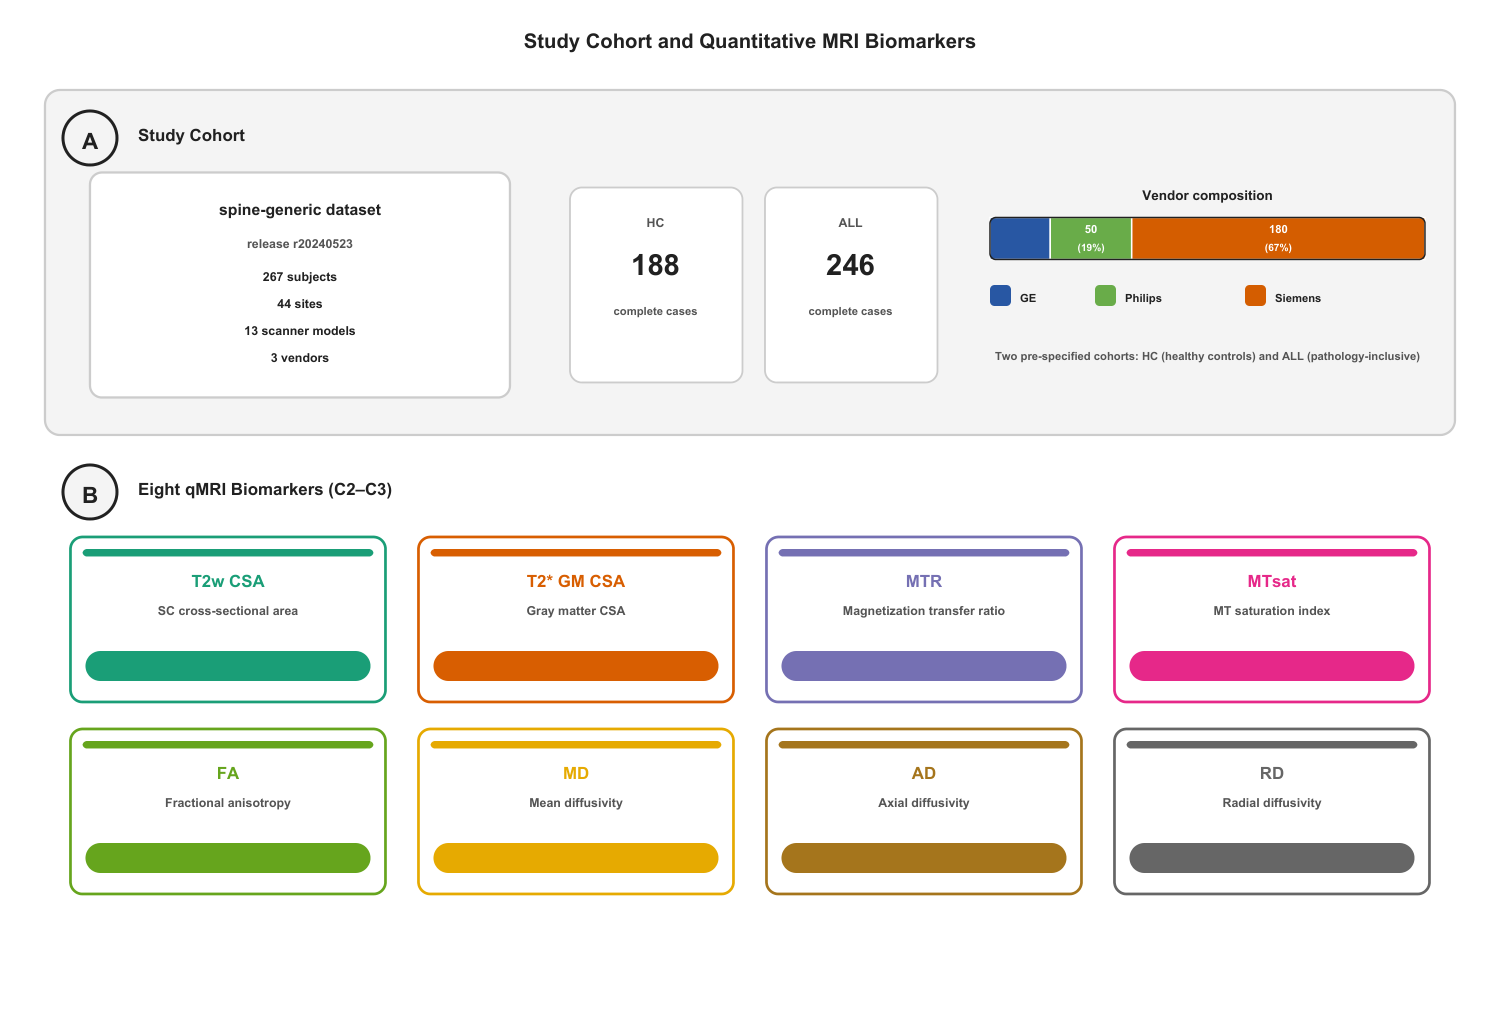
\includegraphics[width=\textwidth]{figures/Fig1a_dataset_biomarkers.png}
\vspace{2mm}
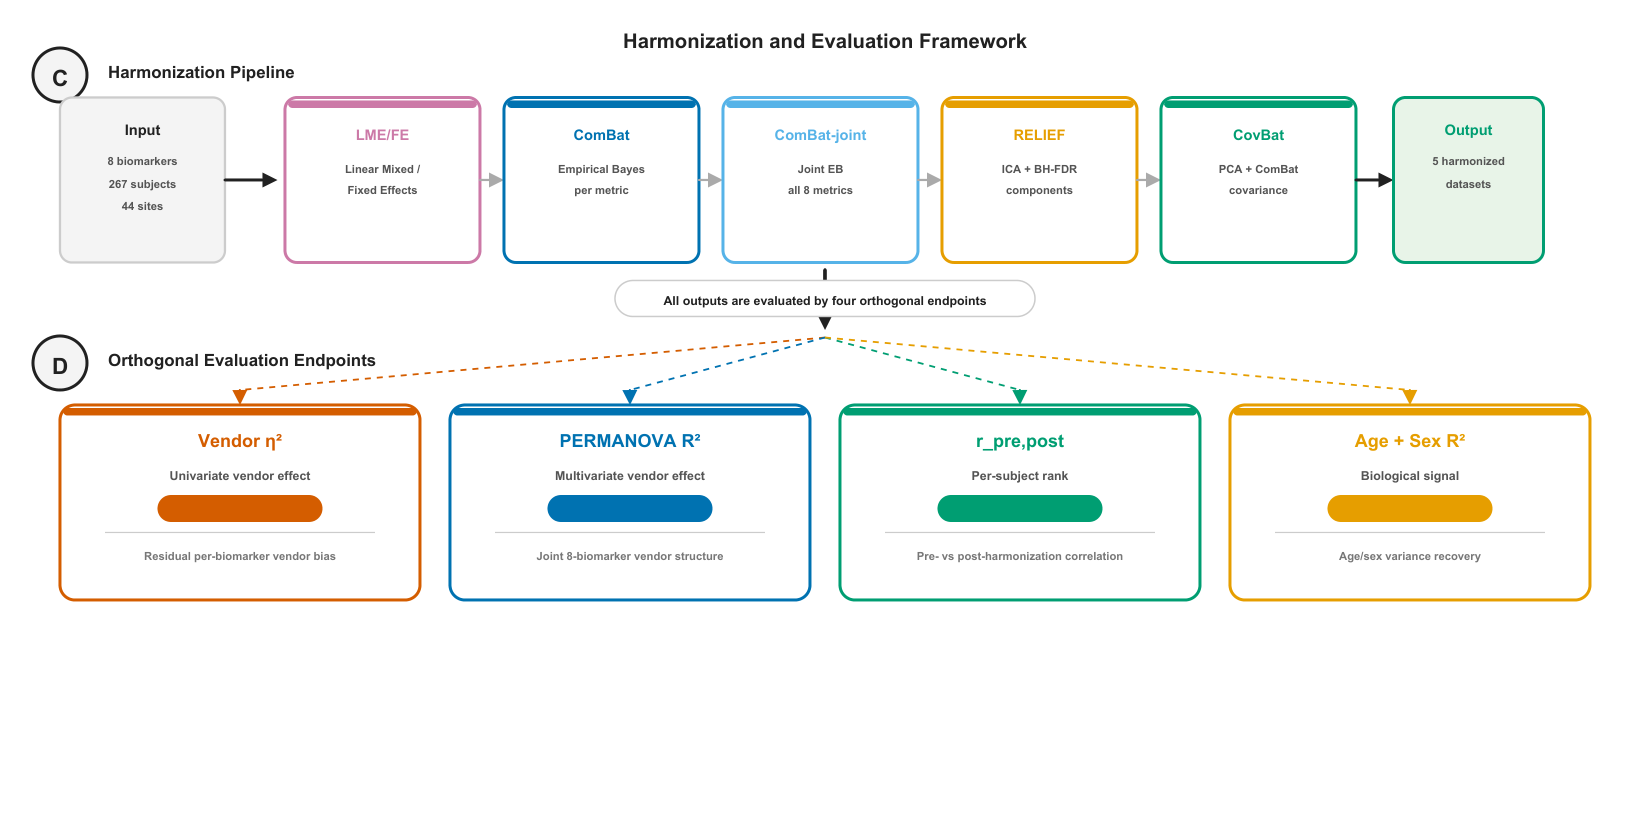
\includegraphics[width=\textwidth]{figures/Fig1b_methods_evaluation.png}
\caption{\textbf{Study design --- data, biomarker extraction, harmonization, and evaluation.} (\textbf{A}) The spine-generic multi-subject dataset: 267 subjects from 44 sites and 13 scanner models across 3 vendors, analyzed in two pre-specified cohorts (HC, $N=188$; ALL, $N=246$). Vendor composition is shown as a stacked bar for the full dataset (GE: 37; Philips: 50; Siemens: 180). (\textbf{B}) Eight qMRI biomarkers extracted at C2--C3 using SCT v6.4, spanning four acquisition families (T2w / T2* / MT / DTI). (\textbf{C}) Five harmonization methods ordered by the breadth of vendor-related variance components they model---from intercept-only (LME/FE) to full covariance+latent-factor correction (CovBat, RELIEF). (\textbf{D}) Three orthogonal evaluation endpoints: vendor-effect removal ($\eta^2$, ICC, PERMANOVA $R^2$), biological-signal recovery (age/sex semi-partial $R^2$), and subject-level preservation (within-vendor pre-post Pearson $r$).}
\label{fig:study_design}
\end{figure}

\subsection{Harmonization Methods}

Five harmonization strategies were applied independently to the biomarker table of each cohort, with \emph{vendor} (GE/Philips/Siemens) as the batch variable and \emph{age} and \emph{sex} as biological covariates to preserve:

\begin{enumerate}[nosep]
  \item \textbf{Per-metric parametric ComBat} \cite{johnson2007adjusting,fortin2017harmonization}: Each biomarker harmonized separately using the location-and-scale model with default parametric EB priors (eb=True), no reference batch, and age/sex preserved through the design matrix. This reflects standard practice when joint multivariate dependence is not explicitly modeled.
  \item \textbf{ComBat-joint} \cite{fortin2017harmonization}: The same model applied jointly to all eight biomarkers simultaneously, so that EB shrinkage borrows information across features within each vendor---the standard brain-imaging configuration.
  \item \textbf{CovBat} \cite{chen2022mitigating}: Extends ComBat by additionally harmonizing the covariance structure: after standard ComBat on mean and variance, residuals are projected into principal-component space (95\% cumulative variance retained), each PC score is itself ComBat-harmonized, and corrected scores are projected back.
  \item \textbf{RELIEF} \cite{zhang2023relief}: Decomposes post-ComBat residuals using FastICA (10 random restarts, best reconstruction-error solution). The pipeline proceeds as: (i) z-score all 8 biomarkers; (ii) apply ComBat to z-scored data; (iii) regress out biological covariates (Age, Sex) to obtain residuals; (iv) PCA retaining 95\% cumulative variance (yielding $K=5$ components); (v) FastICA on $K$-dimensional PC scores to extract $K$ independent components; (vi) for each component, one-way ANOVA $F$-test against vendor, with Benjamini--Hochberg FDR correction ($q < 0.05$ threshold); (vii) zero out batch-loaded components and reconstruct. In practice, no component reached significance in either cohort (all $q \geq 0.99$), so no ICA component was zeroed out. Nevertheless, RELIEF's output differs from standalone ComBat because the pipeline applies additional transformations---covariate regression (step iii), PCA dimensionality reduction (step iv), and the ICA forward--inverse round-trip (steps v--vii)---that reshuffle residual variance even when no component is removed. The net effect is that RELIEF behaves as a mildly regularized variant of ComBat rather than an identical copy, consistent with ComBat already eliminating the bulk of vendor-associable latent structure.
  \item \textbf{LME/FE (random intercept / fixed-effects hybrid)}: A linear mixed-effects model per biomarker, with age, sex, and an intercept as fixed effects and vendor as a random intercept. The harmonized value = original value $-$ EB estimate of the vendor random effect. Because only 3 vendor levels are available---below the $k \geq 5$ recommended for stable variance-component estimation---singular fits are expected. When REML estimation fails (boundary convergence), the method falls back to a fixed-effects OLS ANCOVA: $y \sim \text{Age} + C(\text{Sex}) + C(\text{Manufacturer})$, with harmonized values computed as $y - (\text{vendor offset} - \text{weighted mean of offsets})$. In practice, 12 of 16 biomarker$\times$cohort combinations (6 of 8 biomarkers in each cohort: T2w\_CSA, GM\_CSA, MTR, MTsat, FA, RD) fell back to the FE ANCOVA path; only MD and AD achieved stable LME fits in both cohorts. The ``LME/FE'' label thus refers to this hybrid approach, and the results reflect a mixture of random-intercept shrinkage (for MD, AD) and fixed-effect centering (for the remaining six biomarkers). We use ``LME/FE'' throughout as a study-specific shorthand for this hybrid approach; the label is not intended as a standardized method name.
\end{enumerate}

The five methods form a natural complexity gradient: \textbf{LME/FE} (mean only) $\rightarrow$ \textbf{ComBat} (+scale) $\rightarrow$ \textbf{ComBat-joint} (+joint EB) $\rightarrow$ \textbf{CovBat} (+covariance) $\rightarrow$ \textbf{RELIEF} (+latent factors). This gradient is the structural basis for the trade-off reported in \S 3.6.

\subsection{Statistical Evaluation Framework}

Harmonization performance was evaluated on three orthogonal axes using the following metrics, each averaged across the eight biomarkers:

\textbf{Univariate vendor effect.} Per biomarker: $\eta^2$ from one-way ANOVA (vendor as grouping factor) and one-way ICC(1,1) $= (\text{MS}_B - \text{MS}_W) / (\text{MS}_B + (\bar{n}-1) \cdot \text{MS}_W)$. Negative ICC indicates between-vendor variance smaller than expected under exchangeable subjects---evidence of successful neutralization.

\textbf{Multivariate vendor effect.} PERMANOVA \cite{anderson2001new} on the standardized 8-dimensional biomarker vector (Euclidean distance, 9{,}999 unrestricted permutations---sufficient given that all post-harmonization $p$-values were $\geq 0.97$, far from the 0.05 threshold), vendor as grouping factor. Reported: pseudo-$F$, $R^2$ (proportion of distance variance explained by vendor), and permutation $p$-value. Euclidean distance was chosen as the primary metric because it operates on z-scored features with unit variance, providing an intuitive measure of multivariate separation. A sensitivity analysis using Mahalanobis distance---which accounts for the covariance structure among biomarkers---was also conducted (see Results).

\textbf{Effect-size estimation and bias correction.} Because the vendor groups are imbalanced (Siemens comprises 67\% of the HC cohort), standard $\eta^2$ from one-way ANOVA can be positively biased. We therefore report $\eta^2$ as the primary estimator (for comparability with prior harmonization literature) but also computed omega-squared ($\omega^2$), a less-biased estimator for imbalanced designs, as a sensitivity check. $\omega^2 = (\text{SS}_B - (k-1)\text{MS}_W) / (\text{SS}_T + \text{MS}_W)$, where $k$ is the number of groups. Additionally, 95\% confidence intervals for key summary statistics (mean $\eta^2$, $r_{\text{pre,post}}$, age $R^2$) were estimated via non-parametric bootstrap (2,000 resamples over the 8 biomarkers with replacement). The analysis is descriptive regarding method ranking: no formal multiple-comparison correction was applied across methods, biomarkers, or endpoints, as the study's objective is to characterize the trade-off structure rather than to confirm pairwise superiority of one method over another.

\textbf{Biological-signal recovery.} Semi-partial $R^2$ per biomarker for age and sex separately, averaged across biomarkers. The model was $y \sim \text{Age} + C(\text{Sex})$ applied identically to pre- and post-harmonization data; vendor was \emph{not} included as a covariate in either case, ensuring an apples-to-apples comparison. Semi-partial $R^2_{\text{age}} = R^2_{\text{full}} - R^2_{\text{Sex only}}$; $R^2_{\text{sex}} = R^2_{\text{full}} - R^2_{\text{Age only}}$. Note that the pre-harmonization age $R^2$ therefore includes any vendor-confounded variance (since vendor is not controlled), which is the intended baseline---harmonization should remove this confounding and reveal the true biological signal.

\textbf{Subject-level preservation.} Pearson $r$ between pre- and post-harmonization values, computed within each vendor and averaged across vendors and biomarkers. $r=1$ indicates perfect preservation of within-vendor subject ranking; $r<1$ indicates that harmonization redistributed subject-level deviations.

\begin{figure}[H]
\centering
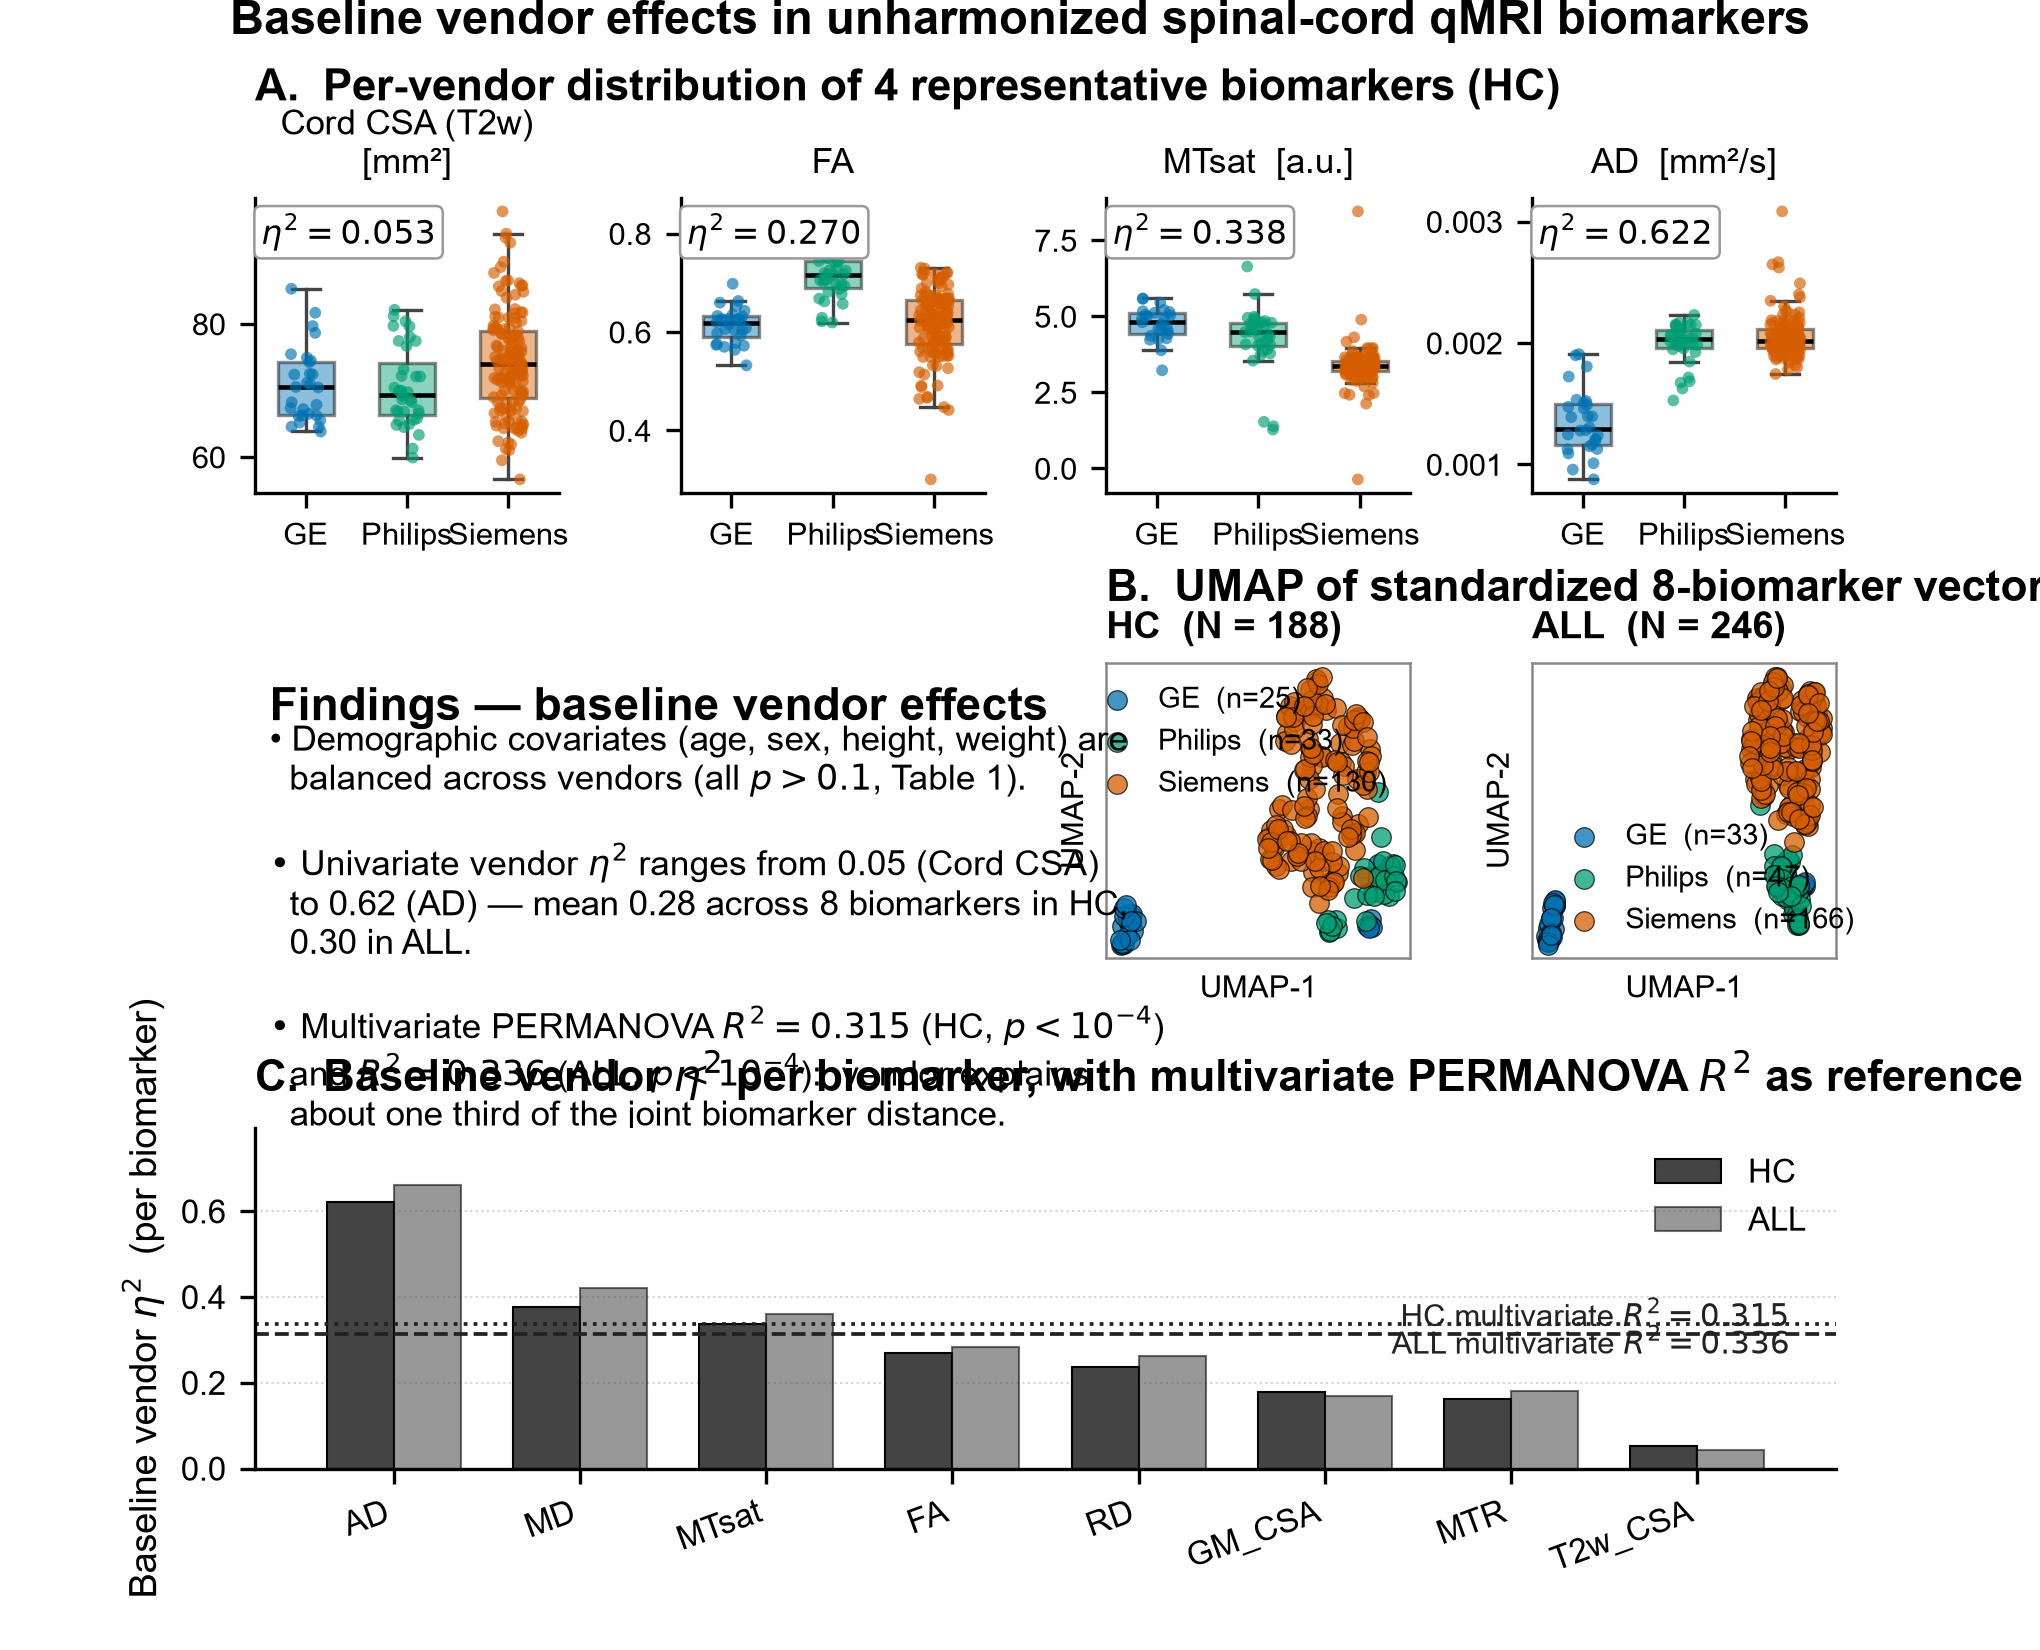
\includegraphics[width=\textwidth]{figures/Fig2_baseline_effects.png}
\caption{\textbf{Baseline vendor effects before harmonization.} (\textbf{A}) Per-vendor distributions of four representative biomarkers spanning the effect-size range: T2w cord CSA ($\eta^2 = 0.05$, smallest effect), FA ($\eta^2 = 0.27$), MTsat ($\eta^2 = 0.34$), and AD ($\eta^2 = 0.62$, largest effect). Systematic vendor offsets are visible in all panels. (\textbf{B}) UMAP projections of the standardized 8-biomarker vector (HC and ALL); vendor clusters are immediately apparent in both cohorts. (\textbf{C}) Per-biomarker baseline vendor $\eta^2$ across all eight biomarkers (HC vs ALL), with PERMANOVA multivariate $R^2$ reference lines (HC $R^2 = 0.315$; ALL $R^2 = 0.336$). Vendor effects range from $\eta^2 = 0.05$ (cord CSA) to $\eta^2 = 0.62$ (AD), exceed age-related variance by $\sim$two orders of magnitude and sex-related variance by $\sim$one order of magnitude, and pervade the multivariate biomarker distribution. $N = 188$ (HC), $N = 246$ (ALL); one-way ANOVA across 3 vendors.}
\label{fig:baseline}
\end{figure}

\subsection{Software and Reproducibility}

All analyses were implemented in Python 3.13. Image processing used SCT v6.4 \cite{deleener2017sct} (the version distributed with the spine-generic processing pipeline; \url{https://spine-generic.readthedocs.io}). Harmonization used \texttt{neuroCombat} 0.2.12, the reference \texttt{CovBat} implementation, an in-house RELIEF implementation using \texttt{scikit-learn} FastICA with BH-FDR control, and \texttt{statsmodels} v0.14 for LME. PERMANOVA was implemented via \texttt{scikit-bio} v0.5 (9999 permutations). UMAP projections used \texttt{umap-learn} 0.5. Figures were rendered with \texttt{matplotlib} 3.8 at 300 dpi (PNG) and as vector PDFs (fonttype=42), using the Wong 2011 color-blind-safe palette and the Arial typeface.

% ===================================================================
\section{Results}

\subsection{Cohort Characteristics}

The HC cohort comprised 203 healthy participants (28 GE / 36 Philips / 139 Siemens; $N = 188$ retained with complete data on all eight biomarkers). Mean age was 28.7 $\pm$ 5.6 years (range 19--52). The pathology-inclusive ALL cohort additionally included participants with mild cervical compression and DCM ($N = 246$ retained with complete data). Full demographic balancing across vendors is documented in Table~\ref{tab:demographics}; pathology distribution was likewise balanced ($\chi^2$ $p = 0.661$). The balanced covariate structure is a necessary precondition: observed vendor effects cannot be attributed to confounding by age, sex, or body habitus.

\subsection{Baseline Vendor-Driven Variance}

Before harmonization, vendor explained a substantial fraction of biomarker variance. Averaged across the eight biomarkers, the vendor effect was $\eta^2 = 0.280 \pm 0.172$ in the HC cohort and $\eta^2 = 0.298 \pm 0.188$ in the ALL cohort, corresponding to a mean ICC(1,1) of $0.345 \pm 0.194$ and $0.367 \pm 0.209$, respectively (Table~\ref{tab:summary}, ``Original'' rows). The vendor effect varied dramatically across biomarkers, from $\eta^2 = 0.05$ for T2w cord CSA (the most vendor-robust metric) to $\eta^2 = 0.62$ for AD (the most vendor-sensitive; Figure~\ref{fig:baseline}). Other diffusion metrics showed intermediate-to-large effects: MD $\eta^2 = 0.38$, FA $\eta^2 = 0.27$, RD $\eta^2 = 0.24$. MT-based metrics showed moderate vendor dependence: MTsat $\eta^2 = 0.34$, MTR $\eta^2 = 0.16$. Gray-matter CSA showed $\eta^2 = 0.18$. In aggregate, roughly one-third of the total variance in the typical biomarker, and as much as 62\% for AD and 30--40\% for MTsat, MD, and FA, was attributable to vendor rather than to inter-subject biology.

\textbf{Sensitivity analyses.} Three sensitivity checks confirmed the robustness of these baseline estimates. (i)~\emph{Per-site sample size:} The 267 subjects were distributed across 44 sites (mean $6.1 \pm 1.9$ subjects/site; range 1--11), with only 4 sites having $n < 5$. Excluding these small sites (retaining 256/267 subjects, 95.9\%) changed the mean vendor $\eta^2$ from 0.298 to 0.314---a negligible difference that does not affect conclusions. (ii)~\emph{Effect-size estimator:} Omega-squared ($\omega^2$), which corrects for positive bias under imbalanced designs, yielded values only $\sim$0.01 lower than $\eta^2$ per biomarker (e.g., AD: $\eta^2 = 0.62$, $\omega^2 = 0.62$; MD: $\eta^2 = 0.38$, $\omega^2 = 0.37$), confirming that imbalance-related bias is minimal. (iii)~\emph{Bootstrap confidence intervals:} The mean vendor $\eta^2$ in the HC cohort was 0.279 [95\% CI: 0.175, 0.397], and the key preservation metrics had CIs that did not overlap between the extreme methods (LME/FE $r = 0.840$ [0.761, 0.903] vs.\ CovBat $r = 0.782$ [0.697, 0.854]), though intermediate methods' CIs overlapped, indicating that the ranking is robust but pairwise differences between adjacent methods should be interpreted as descriptive rather than confirmatory.

Multivariate analysis reinforced and extended the univariate findings. PERMANOVA on the standardized 8-dimensional biomarker vector returned $R^2 = 0.315$ in HC (pseudo-$F = 42.5$, $p < 10^{-4}$) and $R^2 = 0.336$ in ALL (pseudo-$F = 61.5$, $p < 10^{-4}$). These multivariate $R^2$ values (0.315--0.336) fall within the range of moderate-to-large univariate effects (individual biomarker $\eta^2$ spanning 0.05--0.62). This demonstrates that vendor differences pervade the joint biomarker distribution---vendor-specific covariance patterns create separation in the full 8-dimensional space. Notably, no single univariate metric fully captures this multivariate vendor structure: the PERMANOVA $R^2$, while substantial, does not exceed the most extreme univariate $\eta^2$ (AD $= 0.62$), confirming that univariate and multivariate metrics capture complementary aspects of vendor influence.

By contrast, the average semi-partial $R^2$ explained by age was only $0.0026 \pm 0.0041$ (HC) and $0.0067 \pm 0.0100$ (ALL), and by sex $0.025 \pm 0.044$ (HC) and $0.022 \pm 0.033$ (ALL). The vendor effect therefore exceeded age-related variance by approximately two orders of magnitude ($\eta^2 = 0.280$ vs.\ age $R^2 = 0.0026$; ratio $\sim 108\times$) and sex-related variance by approximately one order of magnitude ($\eta^2 = 0.280$ vs.\ sex $R^2 = 0.025$; ratio $\sim 11\times$) in the HC cohort, providing a compelling quantitative motivation for harmonization.

\subsection{Univariate Vendor-Effect Removal}

All five harmonization methods produced an essentially complete univariate decontamination. Across the eight biomarkers, mean vendor $\eta^2$ was reduced by approximately three orders of magnitude in both cohorts (Table~\ref{tab:summary}). In the HC cohort, $\eta^2$ fell from 0.280 (Original) to $3.8 \times 10^{-4}$ (ComBat), $4.9 \times 10^{-4}$ (ComBat-joint), $2.5 \times 10^{-4}$ (CovBat), $4.4 \times 10^{-4}$ (RELIEF), and $3.1 \times 10^{-4}$ (LME/FE)---a reduction of 99.83\%--99.91\%. The corresponding ICC values became slightly negative ($-0.0148$ to $-0.0158$ in HC), confirming that residual between-vendor variance was indistinguishable from---and slightly smaller than---the chance-level expectation under exchangeable subjects. Equivalent magnitudes were observed in the ALL cohort (mean $\eta^2$ reduced from 0.298 to $1.6$--$3.0 \times 10^{-4}$).

Although the five methods are operationally distinct, their univariate residuals were quantitatively similar (all within a factor of 2), reflecting that every method correctly absorbs the dominant location-and-scale vendor offsets. This held with and without pathological subjects, confirming that the harmonizers were not destabilized by disease cases sharing scanners with controls.

\subsection{Multivariate Vendor Structure (PERMANOVA)}

A more stringent test is whether vendor structure persists in the \emph{joint} biomarker distribution after correction---methods that aggressively shrink per-metric means can leave vendor-specific covariance patterns intact. PERMANOVA results (Figure~\ref{fig:performance}) directly addressed this.

\begin{figure}[H]
\centering
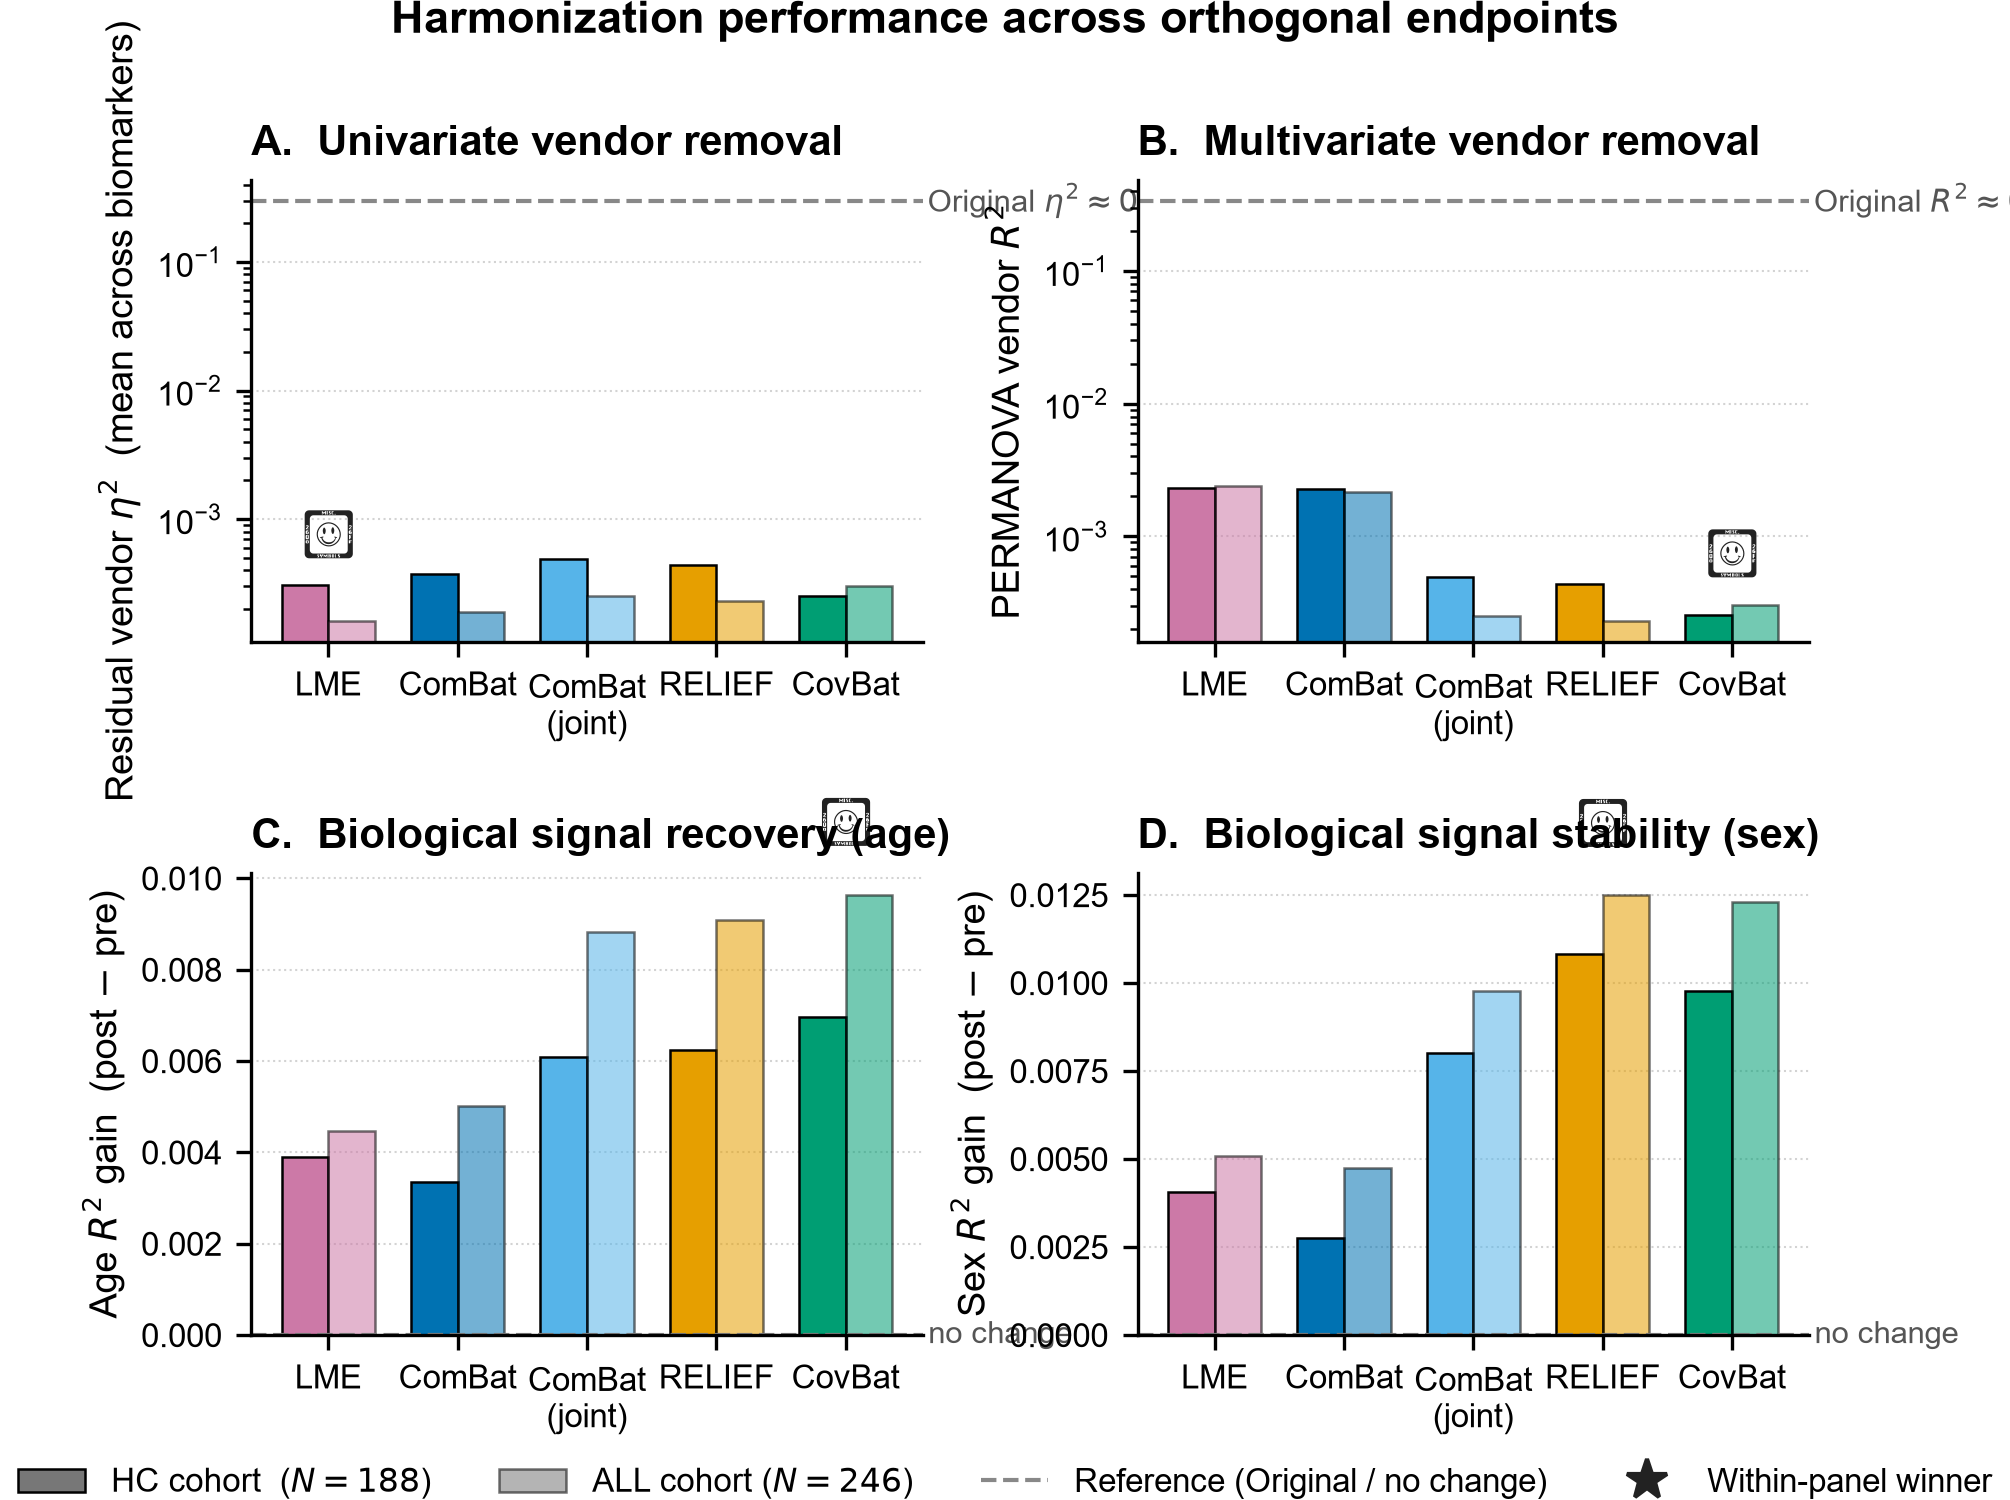
\includegraphics[width=\textwidth]{figures/Fig3_performance.png}
\caption{\textbf{Harmonization performance across evaluation endpoints.} Results shown jointly for HC ($N=188$) and ALL ($N=246$) cohorts. (\textbf{A}) Mean univariate vendor effect ($\log_{10} \eta^2$); baseline values as dashed reference lines. All five methods achieve a $>3$-order-of-magnitude reduction. (\textbf{B}) Multivariate vendor structure ($\log_{10}$ PERMANOVA $R^2$); all post-harmonization $R^2$ values are $<2.5 \times 10^{-3}$ and all $p$-values $\geq 0.97$. (\textbf{C}) Age semi-partial $R^2$ averaged across biomarkers---every method increases age signal relative to baseline (biology signal recovery). (\textbf{D}) Sex semi-partial $R^2$. Methods ordered by subject-level preservation rank (LME/FE $>$ ComBat $>$ ComBat-joint $>$ RELIEF $>$ CovBat; ``LME'' in the figure labels refers to the hybrid LME/FE approach described in \S~2.3). The star ($\star$) marks the top-performing method per panel. $\eta^2$ and ICC computed via one-way ANOVA across 3 vendors; PERMANOVA via 9,999 permutations, Euclidean distance on z-scored 8-biomarker vectors.}
\label{fig:performance}
\end{figure}

In both cohorts, the baseline multivariate vendor structure was overwhelming (HC: $R^2 = 0.315$, $p < 10^{-4}$; ALL: $R^2 = 0.336$, $p < 10^{-4}$). After harmonization, all five methods reduced the multivariate $R^2$ by more than two orders of magnitude. In the HC cohort, post-harmonization $R^2$ ranged from $2.5 \times 10^{-4}$ (CovBat) to $2.3 \times 10^{-3}$ (ComBat, LME/FE), corresponding to permutation $p$-values of 0.99 (ComBat and LME/FE) or 1.00 (CovBat, ComBat-joint, RELIEF). The ALL cohort showed the same pattern ($R^2$ from $2.3 \times 10^{-4}$ to $2.4 \times 10^{-3}$; all $p \geq 0.97$).

Two observations merit emphasis. First, all methods---including the simple LME/FE random-intercept model---were sufficient to render the multivariate vendor signal statistically indistinguishable from chance, indicating that the dominant multivariate vendor structure is already captured by per-metric mean-and-scale correction. Second, methods that explicitly model covariance (CovBat) or latent factors (RELIEF) achieved the smallest residual $R^2$ values; however, the absolute differences across methods were small ($<2 \times 10^{-3}$), and from a statistical-significance perspective, methods were equivalent on this axis.

\textbf{Distance-metric sensitivity.} To verify that the Euclidean PERMANOVA results were not an artifact of the distance metric, we repeated the baseline HC analysis using Mahalanobis distance, which accounts for inter-biomarker covariance. The Mahalanobis $R^2 = 0.182$ ($F = 20.5$, $p = 0.0002$) was lower than the Euclidean $R^2 = 0.315$ but remained highly significant, confirming that vendor structure pervades the joint biomarker distribution regardless of distance metric. The lower Mahalanobis $R^2$ reflects the fact that some vendor separation is encoded in covariance patterns that Mahalanobis partially absorbs; the persistence of significance under both metrics reinforces the conclusion that vendor effects are multivariate, not merely univariate.

\subsection{Recovery of Biological Signal}

Effective vendor removal would be of little value if it concomitantly erased biological variance. We therefore examined age and sex semi-partial $R^2$ before and after harmonization (Table~\ref{tab:summary}, Figure~\ref{fig:performance}C--D).

Rather than degrading biological signal, every method \emph{increased} the age-related variance explained. In the HC cohort, mean age $R^2$ rose from 0.0026 (Original) to 0.0059 (ComBat), 0.0087 (ComBat-joint), 0.0095 (CovBat), 0.0088 (RELIEF), and 0.0065 (LME/FE)---a 2.3- to 3.7-fold increase (absolute increment: 0.33--0.69 percentage points). The effect was even more pronounced in the ALL cohort (age $R^2$ from 0.0067 to 0.0111--0.0163, a 1.7- to 2.4-fold increase, absolute increment 0.44--0.96 percentage points). Sex variance explained showed a smaller but consistent increase (HC: $0.025 \rightarrow 0.028$--$0.036$; ALL: $0.022 \rightarrow 0.027$--$0.035$).

This improvement in biological-signal detectability is the expected consequence of removing a confounder that, in the unharmonized data, was correlated with vendor-imbalanced biological covariates and partially absorbing their effect. Critically, the largest gains in age-signal recovery were observed with covariance- and ICA-based methods (CovBat $>$ RELIEF $\approx$ ComBat-joint $>$ ComBat $>$ LME/FE), suggesting that part of the biological variance in spinal cord biomarkers is encoded in cross-feature covariation that simpler per-feature models leave entangled with the vendor offset.

\subsection{Subject-Level Preservation and Method Trade-offs}

While vendor-removal and biology-recovery metrics were qualitatively similar across methods, the methods diverged meaningfully on \emph{within-vendor} preservation of subject-level ranking, quantified as the Pearson $r$ between pre- and post-harmonization values within each vendor, averaged across vendors and biomarkers (Table~\ref{tab:summary}; Figures~\ref{fig:tradeoff}, \ref{fig:heatmap}).

\begin{figure}[H]
\centering
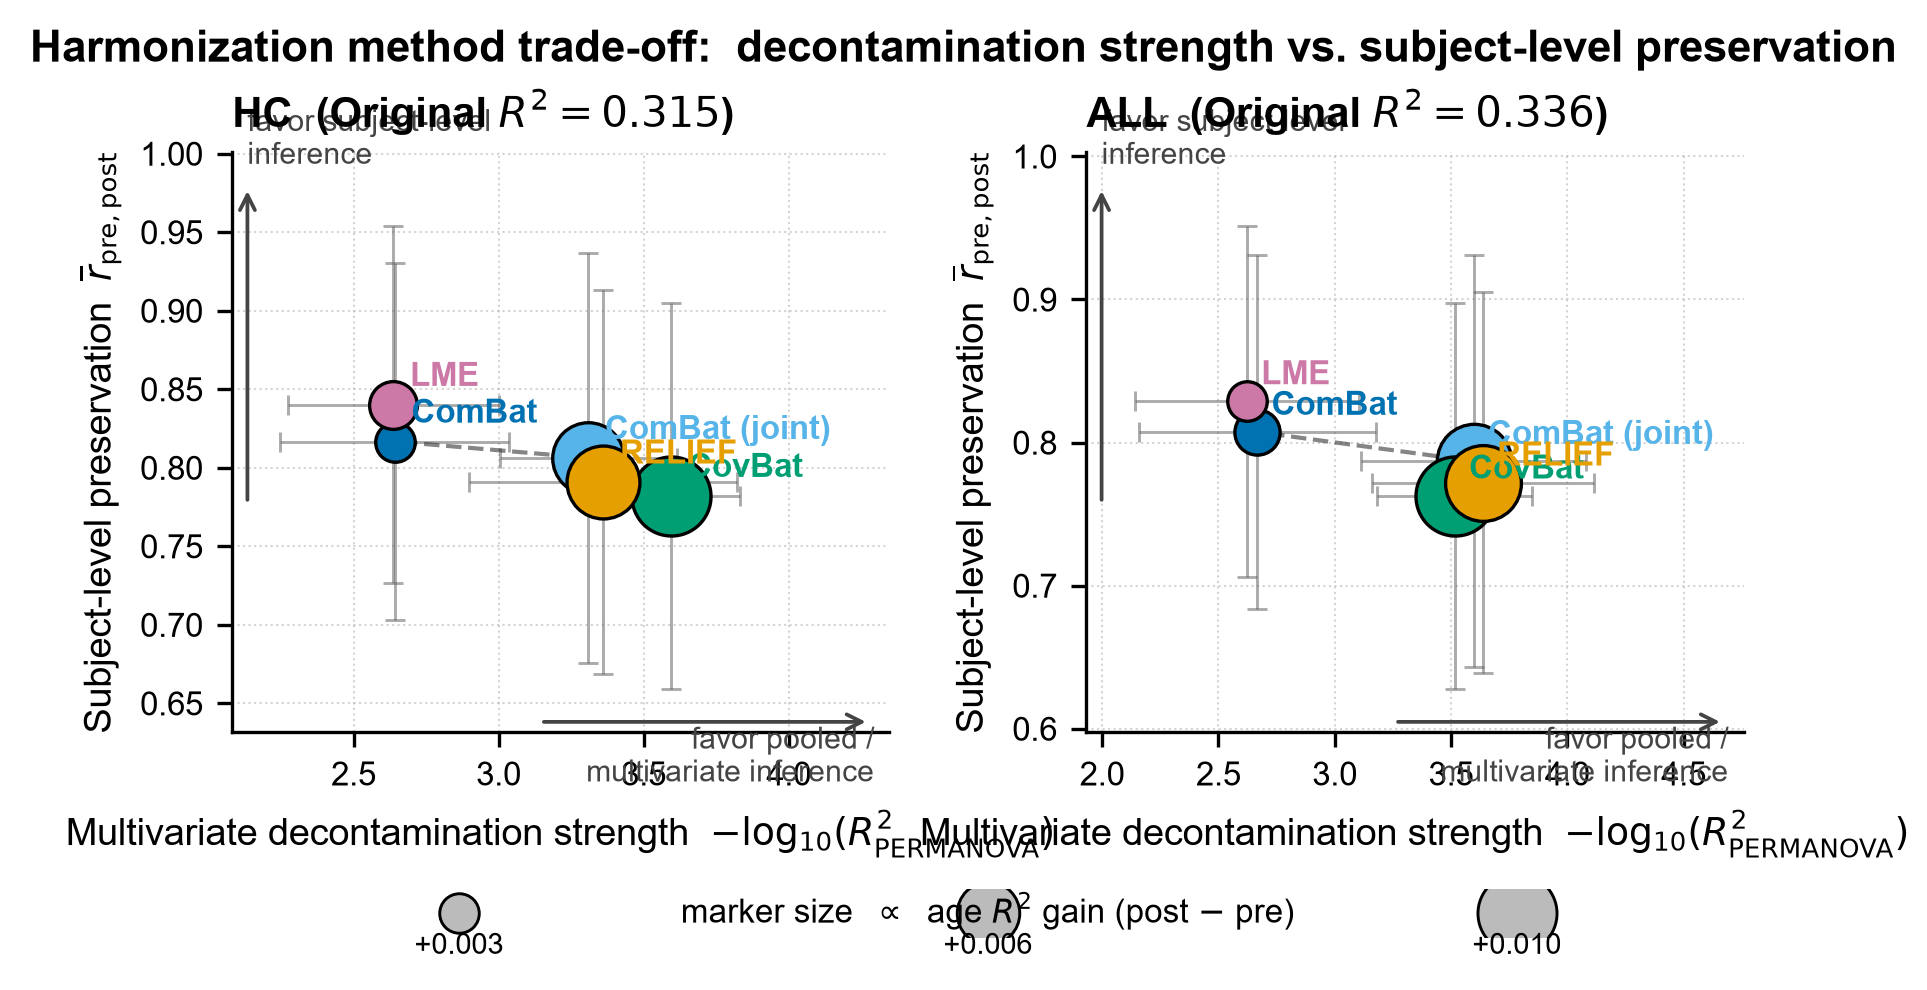
\includegraphics[width=0.95\textwidth]{figures/Fig4_tradeoff.png}
\caption{\textbf{Central trade-off of harmonization.} Each point represents one harmonization method in the plane spanned by multivariate vendor decontamination strength ($-\log_{10}$ PERMANOVA $R^2$; $x$-axis) and within-vendor subject-level preservation (mean $r_{\text{pre,post}}$; $y$-axis). Marker size encodes age $R^2$ gain (biology signal recovery). The Pareto front (dashed line) connects non-dominated methods. LME/FE and per-metric ComBat occupy the high-preservation end of the trade-off; CovBat, RELIEF, and ComBat-joint trade preservation for stronger multivariate decontamination. This plot provides the actionable decision rule: \emph{choose LME/FE or ComBat for subject-level inference; choose CovBat/RELIEF for pooled-group analyses}.}
\label{fig:tradeoff}
\end{figure}

In the HC cohort, LME/FE achieved the highest preservation ($\bar{r} = 0.840 \pm 0.114$), followed by per-metric ComBat ($0.817 \pm 0.114$), ComBat-joint ($0.806 \pm 0.130$), RELIEF ($0.791 \pm 0.122$), and CovBat ($0.782 \pm 0.123$). The same rank order held in the ALL cohort: LME/FE (0.829) $>$ ComBat (0.807) $>$ ComBat-joint (0.787) $>$ RELIEF (0.772) $>$ CovBat (0.763). Differences were modest in absolute terms ($\sim 0.06$ in mean $r$) but consistent across cohorts and biomarkers, indicating a systematic trade-off rather than noise.

\begin{figure}[H]
\centering
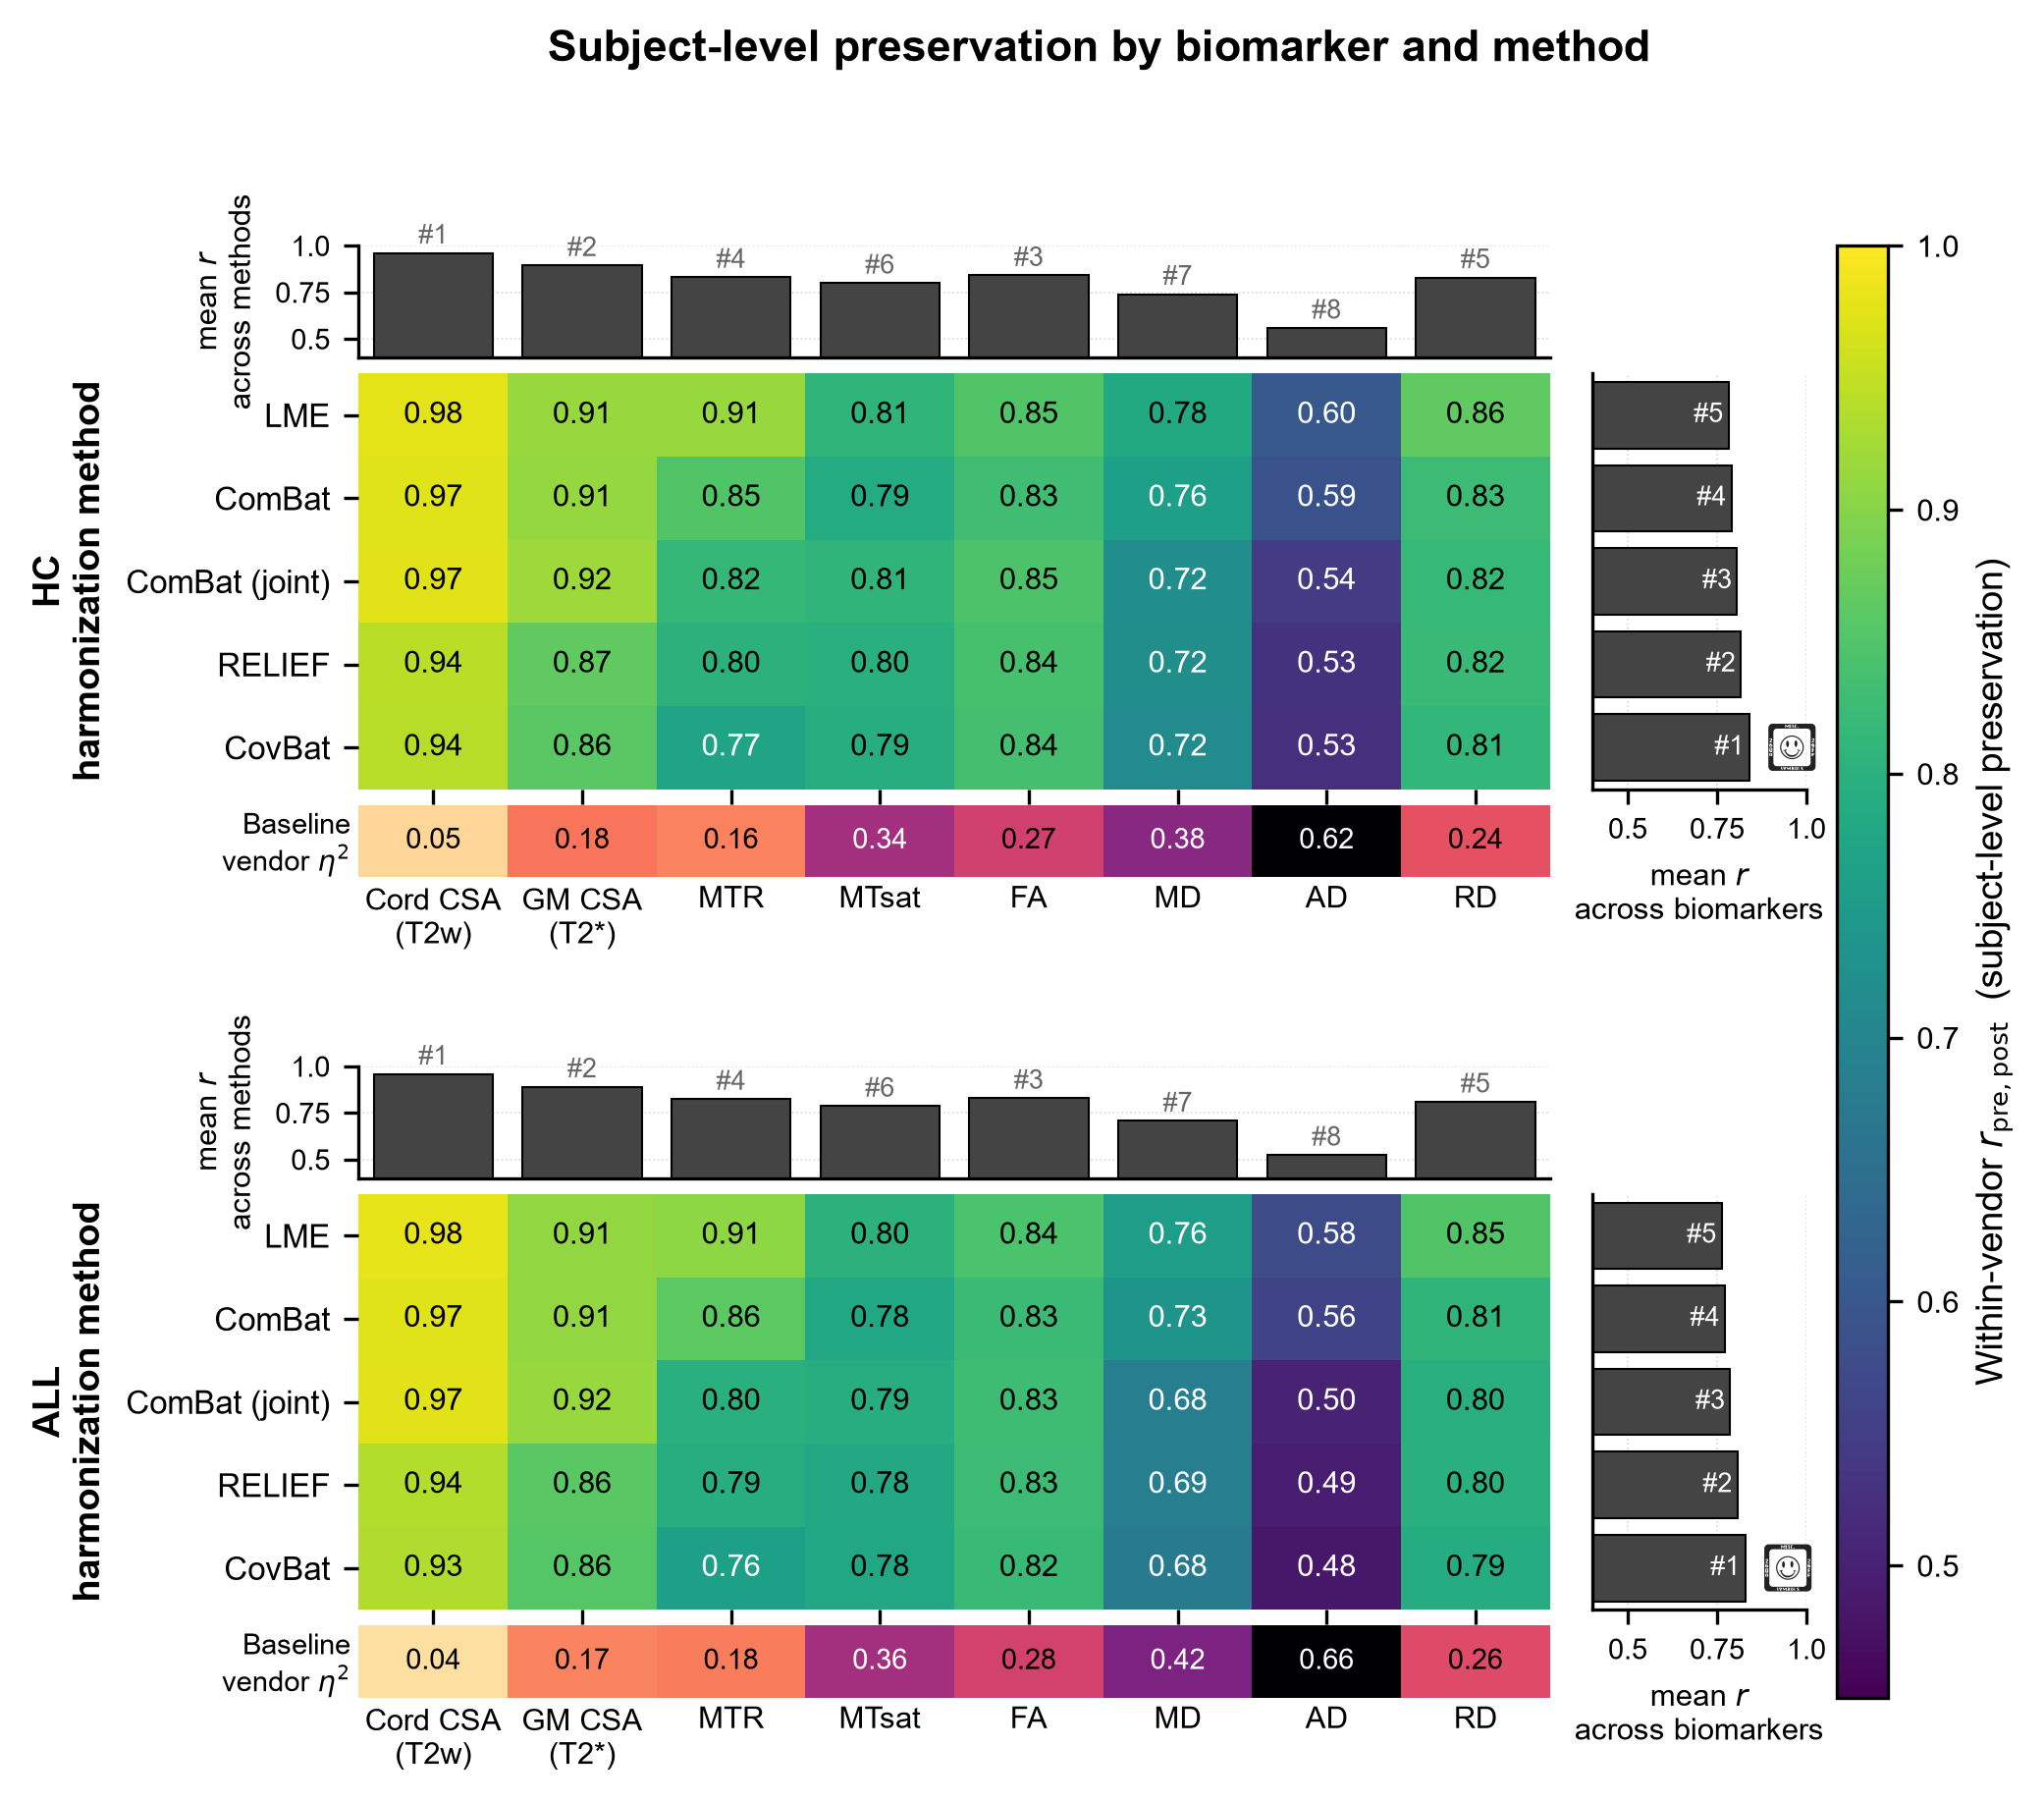
\includegraphics[width=\textwidth]{figures/Fig5_rpre_post_marginals.png}
\caption{\textbf{Subject-level preservation by biomarker and method.} Within-vendor Pearson $r$ between pre- and post-harmonization values, shown as a heatmap for 5 methods (rows) $\times$ 8 biomarkers (columns), separately for HC and ALL cohorts. Cell values are annotated. The top marginal bar shows per-biomarker mean $r$ (revealing that T2w cord CSA is consistently best preserved, $r \geq 0.93$, while AD is the most challenging, $r = 0.48$--$0.60$). The right marginal bar shows per-method mean with rank (\#1--\#5). The bottom strip (magma color scale) shows baseline vendor $\eta^2$ per biomarker, making the inverse correspondence immediately visible: biomarkers with the largest baseline vendor effects are the ones most affected by harmonization.}
\label{fig:heatmap}
\end{figure}

\begin{table}[H]
\centering
\caption{Cohort-level harmonization summary. Each cell is the mean across the eight biomarkers.\newline
Vendor $\eta^2$ and ICC: smaller is better (ICC may be slightly negative under successful neutralization).\newline
Age/sex $R^2$: higher is better (biology signal recovery).\newline
$r_{\text{pre,post}}$: within-vendor Pearson $r$, higher is better (subject-level preservation).}
\label{tab:summary}
\begin{tabular}{llccccc}
\toprule
\textbf{Cohort} & \textbf{Method} & \textbf{Vendor $\eta^2$} & \textbf{Vendor ICC} & \textbf{Age $R^2$} & \textbf{Sex $R^2$} & \textbf{$r_{\text{pre,post}}$} \\
\midrule
\multirow{6}{*}{HC} & Original      & 0.2795 & +0.345 & 0.0026 & 0.0254 & 1.000 \\
                     & ComBat        & $3.8\times10^{-4}$ & $-$0.0148 & 0.0059 & 0.0282 & \textbf{0.817} \\
                     & ComBat-joint  & $4.9\times10^{-4}$ & $-$0.0155 & 0.0087 & 0.0334 & 0.806 \\
                     & CovBat        & $2.5\times10^{-4}$ & $-$0.0158 & \textbf{0.0095} & \textbf{0.0352} & 0.782 \\
                     & RELIEF        & $4.4\times10^{-4}$ & $-$0.0156 & 0.0088 & 0.0362 & 0.791 \\
                     & LME/FE$^\dagger$ & $3.1\times10^{-4}$ & $-$0.0149 & 0.0065 & 0.0295 & \textbf{0.840} $\star$ \\
\midrule
\multirow{6}{*}{ALL}& Original      & 0.2977 & +0.367 & 0.0067 & 0.0223 & 1.000 \\
                     & ComBat        & $1.9\times10^{-4}$ & $-$0.0114 & 0.0117 & 0.0270 & \textbf{0.807} \\
                     & ComBat-joint  & $2.5\times10^{-4}$ & $-$0.0120 & 0.0155 & 0.0320 & 0.787 \\
                     & CovBat        & $3.0\times10^{-4}$ & $-$0.0119 & \textbf{0.0163} & \textbf{0.0346} & 0.763 \\
                     & RELIEF        & $2.3\times10^{-4}$ & $-$0.0120 & 0.0157 & 0.0348 & 0.772 \\
                     & LME/FE$^\dagger$ & $1.6\times10^{-4}$ & $-$0.0115 & 0.0111 & 0.0273 & \textbf{0.829} $\star$ \\
\bottomrule
\end{tabular}
\vspace{4pt}
\par\small\textit{Note:} $\star$ marks the best preservation method. $^\dagger$LME/FE = hybrid approach: random-intercept LME where REML convergence was stable (MD, AD), fixed-effects ANCOVA fallback otherwise (6 of 8 biomarkers); see \S~2.3 for details. All five methods reduce vendor $\eta^2$ by $>99.8\%$ and increase biological signal recovery relative to baseline. Bootstrap 95\% CIs (2,000 resamples over 8 biomarkers) for key HC metrics: vendor $\eta^2$---Original 0.279 [0.175, 0.397], all post-harmonization methods $< 0.001$; $r_{\text{pre,post}}$---LME 0.840 [0.761, 0.903], ComBat 0.817 [0.738, 0.886], CovBat 0.782 [0.697, 0.854]; age $R^2$---Original 0.0026 [0.0004, 0.0060], CovBat 0.0095 [0.0018, 0.0196]. CIs for adjacent methods on $r_{\text{pre,post}}$ overlap, indicating the ranking is robust but pairwise differences between neighboring methods should be interpreted descriptively. A per-biomarker supplementary table (Table~S1) providing all metrics for all 8 biomarkers $\times$ 5 methods $\times$ 2 cohorts is available in the Supplementary Materials.
\end{table}

The per-biomarker breakdown (Figure~\ref{fig:heatmap}) reveals a striking inverse correspondence: biomarkers with the largest baseline vendor effects are the hardest to preserve after harmonization. T2w cord CSA---the least vendor-affected metric ($\eta^2 = 0.05$)---is preserved with $r \geq 0.93$ by every method. AD---the most vendor-affected ($\eta^2 = 0.62$)---shows the largest post-harmonization redistribution: $r$ ranges from 0.48--0.50 for CovBat/ComBat-joint/RELIEF to 0.56--0.60 for ComBat/LME/FE in the ALL cohort. This pattern is exactly what one expects from a principled correction: the metric most corrupted by vendor carries the largest required correction, and the metric least affected by vendor is modified the least.

Crucially, \emph{all} methods achieved within-vendor Pearson $r > 0.75$ for the average biomarker, meaning that downstream analyses ranking subjects within a vendor (e.g., clinical thresholding, percentile-based abnormality detection) remain valid after any of the five harmonizations.

\subsection{Design C: Balanced Subsampling Robustness Analysis (Supplementary)}

To evaluate whether the Siemens-dominated sample composition (67\% of HC cohort) influenced the preservation ranking, we conducted a supplementary balanced-subsample analysis (Design C; Figure~\ref{fig:designC}). Twenty independent random seeds were used to subsample Siemens subjects to parity with GE+Philips, yielding balanced cohorts of $n \approx 98$ per seed. Harmonization was re-applied identically.

\begin{figure}[H]
\centering
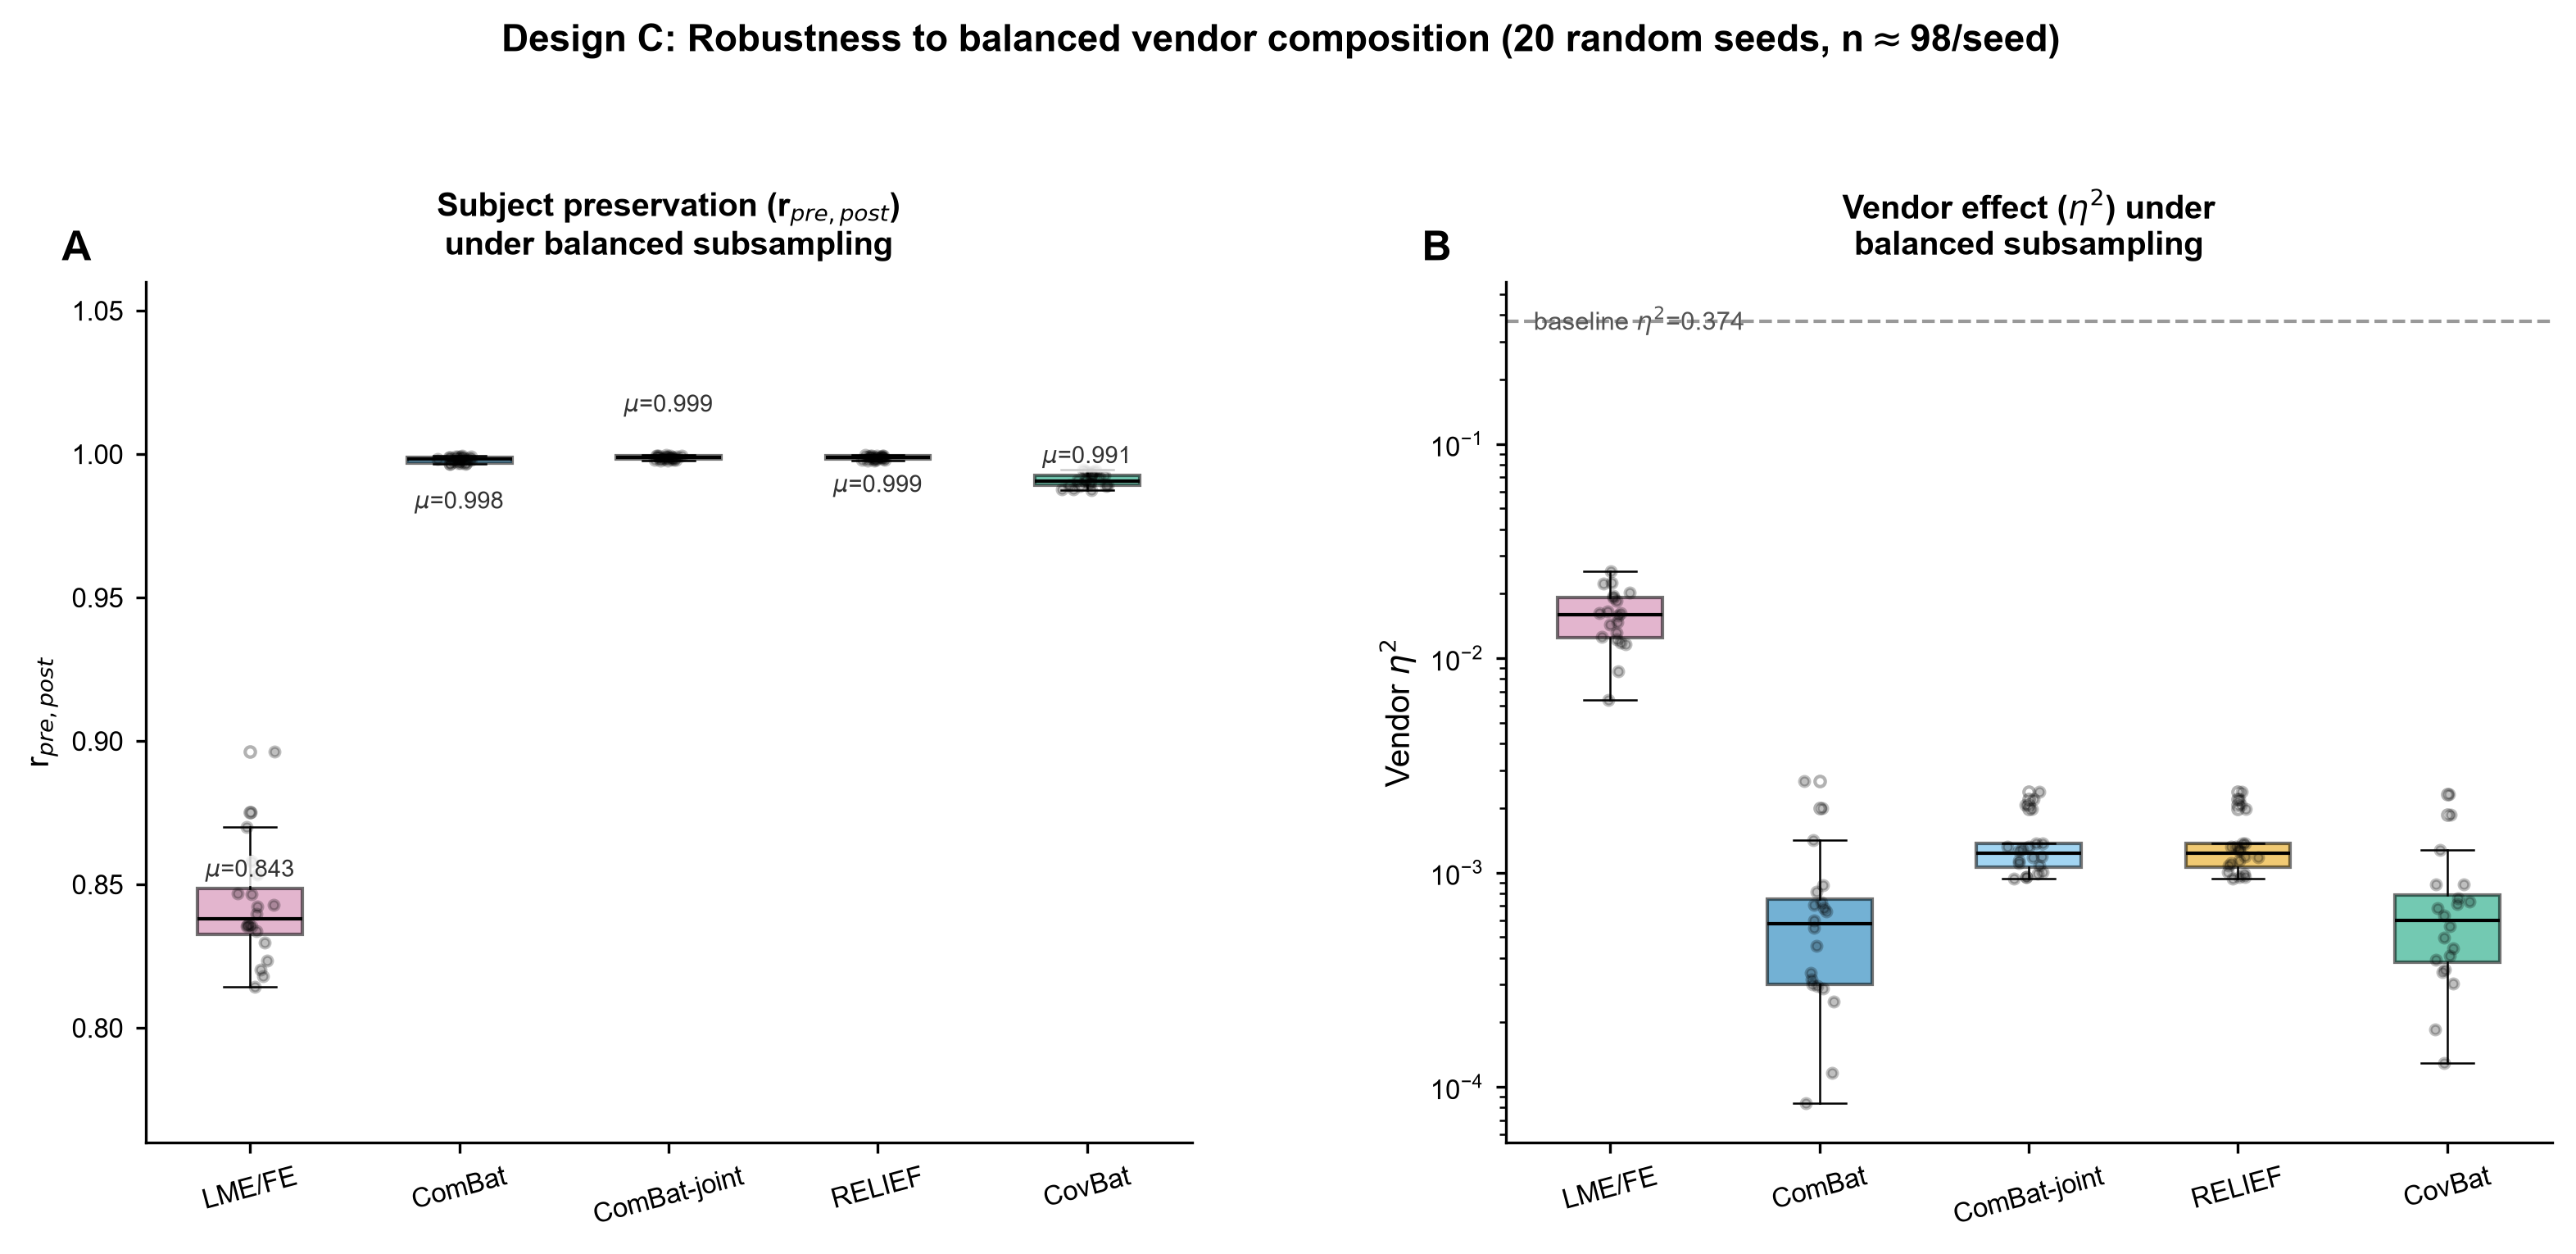
\includegraphics[width=\textwidth]{figures/FigS_design_C_robustness.png}
\caption{\textbf{(Supplementary) Design C: Balanced subsample robustness analysis.} Under balanced vendor composition (Siemens downsampled to parity), all methods except LME/FE achieve nearly perfect subject preservation ($r \geq 0.991$ for CovBat, $r \geq 0.998$ for others). This confirms that the preservation ranking in the main analysis (LME/FE $>$ ComBat $>$ \dots $>$ CovBat) reflects the asymmetry of the full cohort: when vendor groups are balanced, even the most aggressive multivariate correction preserves individual rankings. Design C values differ from the main results and should be interpreted as a robustness confirmation---not as a substitute for the primary analysis.}
\label{fig:designC}
\end{figure}

Under balanced conditions, all methods except LME/FE achieved nearly perfect subject preservation (CovBat: mean $r = 0.991$; ComBat/ComBat-joint/RELIEF: $r \geq 0.998$; LME/FE: $r = 0.841$). This confirms that the preservation gradient observed in the main analysis reflects the real-world asymmetry of vendor representation, not an intrinsic limitation of the methods. In balanced consortia, aggressive covariance correction (CovBat) can be deployed with minimal preservation penalty.

% ===================================================================
\section{Discussion}

\subsection{Principal Findings}

\noindent\fbox{\parbox{0.95\textwidth}{
\textbf{Summary of principal findings:}\\[4pt]
(1) Vendor explains $\sim$28\% of univariate biomarker variance and $\sim$32\% of multivariate structure---exceeding age-related variance by $\sim$two orders of magnitude and sex-related variance by $\sim$one order of magnitude.\\
(2) All five methods reduce vendor effects to statistical negligibility ($\eta^2 < 5 \times 10^{-4}$, PERMANOVA $p \geq 0.97$).\\
(3) Harmonization improves biological-signal detectability: age $R^2$ increases 2.3- to 3.7-fold (though absolute effects remain $<1\%$ of variance).\\
(4) Methods occupy a reproducible Pareto frontier between multivariate decontamination and subject-level preservation (LME/FE or ComBat for subject-level; CovBat/RELIEF for pooled-group analyses).
}}

\vspace{6pt}
In this systematic comparison of statistical harmonization methods applied to spinal cord qMRI biomarkers, four findings are clear and mutually reinforcing.

\textbf{First, vendor is the dominant non-biological source of variance.} The baseline vendor effect---a mean $\eta^2$ of 0.28--0.30 across eight biomarkers, and a PERMANOVA $R^2$ of 0.32--0.34---means that approximately one-third of all biomarker information in a pooled multi-vendor cohort is attributable to the scanner rather than to the subject. For AD, this fraction reaches 62\%. This magnitude makes harmonization not merely advisable but \emph{strongly recommended} for any defensible pooled cross-vendor analysis.

\textbf{Second, all methods work---and their near-equivalence on the primary endpoint is itself an informative result.} Every method tested, including the simplest LME/FE model that removes only per-vendor mean shifts, reduced univariate vendor variance by approximately three orders of magnitude and rendered the multivariate vendor signal indistinguishable from chance (all PERMANOVA $p \geq 0.97$). This convergence is not a limitation but a finding: it demonstrates that the dominant vendor-effect structure in spinal cord qMRI biomarkers is captured by the location-and-scale components that all methods share. The more complex methods (CovBat, RELIEF) add covariance and latent-factor correction that are, for these biomarkers, marginal relative to the large mean shifts they also address. This has an important practical implication: harmonization of spinal cord qMRI does not require the full complexity of the method arsenal---a well-specified linear model (LME/FE) or standard ComBat already eliminates the vast majority of vendor contamination. The choice among methods should therefore be based not on ``which removes vendor effects best''---they all do---but on secondary considerations such as subject preservation and biological-signal recovery.

\textbf{Third, harmonization consistently improves---and never degrades---biological-signal detectability.} Every method was associated with a monotonic increase in age and sex semi-partial $R^2$ relative to baseline: age signal rose 2.3- to 3.7-fold (absolute increment 0.33--0.96 percentage points), and sex signal rose 1.1- to 1.6-fold. The directional consistency---all five methods, both cohorts, both biological covariates---is the scientifically informative result, as it rules out the concern that harmonization might inadvertently absorb biological variance. We caution that the absolute age-related variance explained remains below 1\% post-harmonization (0.65--1.63\% depending on method and cohort). This magnitude is expected given three well-characterized factors: (i) the restricted age range of the spine-generic cohort (19--52 years), which limits the total age-related signal available for any method to recover; (ii) the known modest sensitivity of single-level C2--C3 scalar metrics to normal aging in mid-adulthood---normative spinal cord atrophy rates are on the order of 0.5--1.0 mm$^2$/year \cite{prados2017spinal}, corresponding to a cumulative effect of $\sim$10--30 mm$^2$ over three decades; and (iii) the well-documented dominance of inter-subject biological variability over age trends in cross-sectional spinal cord cohorts of this size. The relevant benchmark is therefore not the absolute magnitude of age $R^2$, but the \emph{fold-change} relative to baseline---which confirms that harmonization unmasks, rather than erases, biological signal. Studies targeting age-related cord changes should consider broader age ranges (e.g., 20--80 years) or multi-level sampling to increase the biological signal pool.

\textbf{Fourth, the methods diverge on subject-level preservation in a reproducible, interpretable manner.} The preservation ranking---LME/FE $>$ ComBat $>$ ComBat-joint $>$ RELIEF $>$ CovBat---is consistent across both cohorts, follows directly from the variance components each method models, and forms a Pareto frontier when plotted against multivariate decontamination strength (Figure~\ref{fig:tradeoff}). This provides an actionable decision framework: choose methods from the high-preservation end of the frontier for subject-level inference (individual prediction, longitudinal change detection, clinical thresholding), and methods from the high-decontamination end for cross-vendor pooled group analyses (case-control separation, cluster analysis, multivariate classification).

\subsection{The Pareto Frontier: A Framework for Method Selection}

A key contribution of this comparison is the observation that harmonization methods do not differ along a single ``better/worse'' axis, but instead occupy a Pareto frontier in the (decontamination, preservation) plane. Formally, a method is \emph{Pareto-optimal} (non-dominated) if no other method achieves both stronger decontamination \emph{and} higher preservation. With only five methods, the frontier was identified by exhaustively checking all pairs: a point is dominated if another point lies above-and-to-the-right of it in the (decontamination, preservation) plane. We note that with five points, the frontier is necessarily a small subset---in our data, all five methods are non-dominated, forming a monotonic trade-off curve. While this is mechanically a ranked scatter plot, the term ``Pareto frontier'' is used to emphasize the structural interpretation: no single method dominates, and the choice depends on the relative weight assigned to each axis. The framework's value lies in its extensibility: as additional methods are evaluated, dominated methods can be identified and pruned, and the frontier sharpens into a genuinely selective tool. This insight reframes the method-selection problem from ``which method is best?'' to ``which method optimizes the endpoint most relevant to my downstream analysis?''

This framing has three practical advantages. First, it is \emph{transparent}: users can see exactly what they are trading when they choose one method over another. Second, it is \emph{goal-dependent}: the same dataset may warrant different harmonization choices depending on whether the planned analysis is subject-level (use LME/FE) or group-level (use CovBat). Third, it is \emph{extensible}: as new harmonization methods are developed, they can be positioned on this same frontier, allowing direct comparison with the existing benchmark.

The mechanistic interpretation follows from the complexity gradient defined in \S~2.3: each additional variance component removed increases multivariate purity at a modest, measurable cost to within-vendor subject ranking. This gradient is not an artifact of our specific dataset---it is a structural property of how these methods operate on multi-feature biomarker vectors.

\subsection{Clinical and Research Implications}

For consortia building pooled spinal cord qMRI resources, our results support three concrete recommendations:

\begin{enumerate}[nosep]
  \item \textbf{Harmonize by default.} The pre-harmonization vendor effect ($\eta^2 \approx 0.28$, PERMANOVA $R^2 \approx 0.32$) is large enough that no defensible pooled group analysis should be performed on raw biomarker values across vendors. The methods evaluated here are computationally lightweight (all run in seconds on a standard laptop for 267 subjects $\times$ 8 biomarkers), freely available, and require no specialized hardware.
  \item \textbf{Match method to inference goal.} Use LME/FE or per-metric ComBat for subject-level analyses (individualized prediction, longitudinal monitoring, clinical decision support). Use ComBat-joint, RELIEF, or CovBat for multivariate pooled-group analyses (disease classification, normative modeling, cross-sectional biomarker discovery).
  \item \textbf{Report the trade-off.} Given the equivalence of methods on vendor-removal but their measurable divergence on subject preservation, we recommend that publications state which axis their method choice optimizes and, ideally, report sensitivity to method choice (e.g., a supplementary table showing key results under two methods from opposite ends of the frontier).
\end{enumerate}

We also note that harmonization was robust to the inclusion of pathological cases. The HC vs ALL comparison showed that adding compression and DCM participants to the harmonization set did not destabilize any method, consistent with the use of biological covariates in the design matrix (which protect against pathological-signal absorption). This supports the standard pipeline of harmonizing the full cohort---including disease cases---before performing disease-specific analyses.

\subsection{Comparison with Brain Imaging Harmonization Literature}

Our results align with and extend findings from the brain imaging harmonization literature. The baseline vendor effect magnitude we observe ($\eta^2 \approx 0.28$) is comparable to---or larger than---site effects reported for cortical thickness (ICC $\approx$ 0.05--0.25) \cite{fortin2018harmonization} and diffusion metrics ($\eta^2 \approx$ 0.10--0.30) \cite{tax2019cross} in brain consortia. The effectiveness of ComBat in spinal cord biomarkers ($\eta^2$ reduction from 0.28 to $\sim 4 \times 10^{-4}$) is at least as strong as its performance in brain diffusion MRI (typically 80--95\% reduction) \cite{fortin2017harmonization,fortin2018harmonization}, and mirrors the inter-scanner agreement improvements recently reported by Middleton et al.\ for spinal cord DTI \cite{middleton2023spinal}. The ComBat best-practice framework of Jodoin et al.\ \cite{jodoin2025combat}---particularly regarding covariate preservation and demographic balance---guided our methodological design and should be consulted by investigators planning spinal cord harmonization pipelines.

The observation that CovBat achieves stronger multivariate decontamination at measurable preservation cost mirrors findings in cortical thickness harmonization \cite{chen2022mitigating}, though the specific trade-off magnitudes are spinal-cord-specific. Our work extends the brain literature in three directions: (i) we provide the first spinal-cord-specific benchmark of the full ComBat-family methods; (ii) we introduce PERMANOVA as a multivariate evaluation endpoint that is more sensitive than per-metric $\eta^2$ to residual vendor structure; and (iii) we formalize the Pareto-frontier framework as a decision tool---an approach that, to our knowledge, has not been applied in prior harmonization benchmarks. These contributions complement existing harmonization guidelines for multicenter MRI \cite{destefano2022magnims} and the recent spinal cord DTI harmonization work of Middleton et al.\ \cite{middleton2023spinal}. Notably, while prior studies have used the spine-generic dataset to establish normative morphometry databases \cite{valosek2024morphometry}, assess longitudinal biomarker stability \cite{boudreau2025longitudinal}, and develop robust segmentation methods \cite{bedard2025contrast}, none has addressed the question of how to statistically harmonize cross-vendor biomarker values for pooled analysis. Our work fills this gap: the normative references of Valo\v{s}ek et al.\ and the reproducibility benchmarks of Boudreau et al.\ characterize biological and temporal variation, whereas we quantify and correct vendor-driven non-biological variation---a complementary and necessary step before these normative and reproducibility frameworks can be applied to multi-vendor pooled cohorts.

\subsection{Relationship to Middleton et al. (2023)}

Because Middleton et al.\ \cite{middleton2023spinal} is the most directly comparable prior work, it merits explicit discussion of how the present study extends---rather than replicates---their findings. Middleton et al.\ demonstrated that longitudinal ComBat harmonization substantially improves inter-scanner agreement for cervical and thoracic spinal cord DTI metrics (FA, MD, AD, RD) in a traveling-subject design. Their work established feasibility and provided an essential proof of concept. Our study differs in design, scope, and analytical framework in ways that are complementary rather than duplicative:

\begin{enumerate}[nosep]
  \item \textbf{Method scope.} Middleton et al.\ evaluated a single harmonization method (longitudinal ComBat); we compare five methods spanning the full complexity gradient from intercept-only (LME/FE) to covariance-plus-latent-factor correction (CovBat, RELIEF). This comparison reveals the \emph{structure} of the vendor effect---that location-scale dominates, and that covariance-level correction provides marginal additional multivariate benefit---which a single-method study cannot address.
  \item \textbf{Biomarker scope.} Middleton et al.\ focused on DTI metrics; we additionally include structural metrics (T2w cord CSA, T2* GM CSA) and magnetization-transfer metrics (MTR, MTsat), which exhibit different vendor-effect profiles ($\eta^2$ ranging from 0.05 for cord CSA to 0.34 for MTsat) and respond differently to harmonization. The inclusion of T2w CSA---the most vendor-robust metric sampled---is particularly important as a negative control.
  \item \textbf{Evaluation framework.} Middleton et al.\ used ICC and coefficient of variation as primary endpoints. We extend evaluation to three orthogonal axes that jointly capture vendor removal, biology recovery, and subject-level preservation. The PERMANOVA endpoint is novel in this context and reveals multivariate vendor structure that univariate ICC cannot detect.
  \item \textbf{Method-selection framework.} Neither Middleton et al.\ nor any prior spinal cord study provided a formal decision framework for method selection. The Pareto-frontier analysis---showing that methods trade multivariate purity for subject-level preservation---is, to our knowledge, the first such quantitative decision tool proposed for spinal cord harmonization.
\end{enumerate}

These differences are not incremental refinements; they reflect fundamentally different study objectives. Middleton et al.\ asked whether ComBat works for spinal cord DTI (it does). We ask which method should be chosen for which downstream goal, and why---a question that requires multi-method, multi-biomarker, multi-endpoint comparison and yields a decision framework applicable beyond the specific dataset studied.

\subsection{Limitations}

Several limitations warrant careful consideration.

\textbf{Vendor-site confounding.} The spine-generic dataset contains 44 sites but only 3 vendors, making it impossible to disentangle vendor effects from site-level effects within each vendor. A systematic Siemens-versus-Philips difference may partially reflect differences in the specific sites operating each vendor's scanners, rather than purely hardware-level differences. This limitation is inherent to the retrospective, multi-vendor design of the spine-generic study and motivates prospective cross-vendor designs with site crossing. Both our findings and their interpretation should be understood as reflecting the composite ``vendor-in-site'' effect, which is the relevant batch unit for most practical multi-center consortia.

\textbf{Limited vendor diversity and imbalance.} The dataset covers only three vendors (GE, Philips, Siemens) and is dominated by Siemens scanners (67\% of HC cohort). The preservation ranking we report may be sensitive to vendor imbalance---as confirmed by our Design C supplementary analysis, which shows that balanced subsampling compresses the preservation difference across methods. Extrapolation to other vendors (e.g., Canon, United Imaging) or to scanner models not represented in this dataset should be undertaken cautiously.

\textbf{Modest biological effect sizes.} Although harmonization consistently increased the age-related variance explained (2.3--3.7 fold relative to baseline), the absolute effect remains small: age explains less than 1\% of post-harmonization biomarker variance, and less than 1.7\% even in the best-case (CovBat, ALL cohort). These small effect sizes partly reflect the limited age range (19--52 years) and the known moderate sensitivity of single-level C2--C3 scalar metrics to normal aging. Studies targeting age-related cord changes should consider broader age ranges or more spatially extended sampling.

\textbf{Method convergence on univariate endpoints.} The $\eta^2$ of all five methods fell within the same narrow range ($\sim 10^{-4}$), giving the methods no meaningful differentiation on the primary endpoint of vendor-effect removal. This convergence means that the study's main comparative dimension---subject-level preservation---is not the direct goal of harmonization, and readers should weigh its practical significance against the near-identical vendor-removal performance of all methods.

\textbf{Absence of external validation.} Our evaluation is entirely internal: we benchmark methods on the same dataset on which they are applied. This does not test generalization to unseen scanners or protocols. The Design C balanced-subsample analysis provides internal robustness evidence, but a true out-of-sample validation (e.g., leave-one-vendor-out cross-validation using ComBat-from-template) would more directly assess real-world deployability.

\textbf{Single-level (C2--C3) assessment.} Our analysis is restricted to a single vertebral level, and results may differ at other cord levels or when using multi-level aggregated metrics. The narrow age range (19--52 years) additionally limits the biological signal available for detecting age-related changes, a factor that likely contributes to the small age $R^2$ values observed.

\textbf{Absence of disease-versus-control separation analysis.} Although the ALL cohort includes participants with mild cervical compression ($n=56$) and DCM ($n=2$), our biological-signal validation relies solely on age and sex semi-partial $R^2$, which explain $<1\%$ of post-harmonization variance. A more clinically impactful validation---testing whether harmonization preserves or improves disease-versus-control separation (e.g., Cohen's $d$, AUC for DCM vs.\ HC classification)---was not performed. The primary reason is statistical power: with only 58 pathology subjects in the complete-case ALL cohort (and only 2 DCM cases), any disease-separation metric would be underpowered and potentially misleading. Additionally, the spine-generic dataset was not designed as a case-control study, and the pathology cases span a severity spectrum that does not map cleanly onto binary classification. Future work using dedicated case-control cohorts with adequate sample sizes should directly evaluate whether harmonization preserves clinically relevant disease signal.

\textbf{Method scope.} Our comparison covers only the ComBat family of methods (including extensions); other approaches (e.g., traveling-subject calibration, generative model-based harmonization) fall outside our scope. Claims about ``optimal'' method selection are therefore relative to the ComBat-family methods tested in this study.

\subsection{Future Directions}

Several directions follow naturally. (i) Prospective out-of-sample evaluation on a held-out vendor using ComBat-from-template implementations will be critical for real-world deployment. (ii) Integration with longitudinal designs will allow direct quantification of how much post-harmonization subject-level deviation reflects information loss versus true biological change. (iii) The reproducible, vendor-correlated covariance structure exploited by CovBat and RELIEF invites explicit modeling: a unified framework that partitions vendor-driven mean, scale, and covariance components might combine LME/FE's high subject preservation with CovBat's multivariate purity. (iv) Extending this benchmark to voxel-level or lesion-level spinal cord biomarkers represents the natural next step toward harmonization of spatial maps for lesion-burden quantification in demyelinating and degenerative disease. (v) Incorporating scanner-model-level harmonization in larger, more balanced consortia would allow a finer-grained decomposition of vendor-versus-model effects.

% ===================================================================
\section{Conclusion}

In a systematic benchmark of five statistical harmonization methods on standardized multi-vendor spinal cord qMRI biomarkers, all methods effectively eliminated vendor variance (reduction to $\sim 10^{-4}$, a $>99.8\%$ decrease) and rendered multivariate vendor structure indistinguishable from chance (every PERMANOVA $p \geq 0.97$). The methods diverge meaningfully only on the trade-off between aggressive multivariate decontamination and preservation of within-vendor subject ranking: LME/FE and per-metric ComBat best preserve subject-level structure ($r \geq 0.82$), while CovBat and RELIEF maximize multivariate purity. This trade-off forms a reproducible Pareto frontier that provides a quantitative, actionable framework for method selection: match the harmonization strategy to the downstream analytic goal. Given the magnitude of baseline vendor effects ($R^2 \sim 0.32$), harmonization should be considered strongly recommended---not optional---for any pooled multi-vendor spinal cord qMRI analysis.

% ===================================================================
\section*{Data and Code Availability}

The spine-generic multi-subject dataset is openly available at \url{https://github.com/spine-generic/data-multi-subject} (release r20240523). All processing scripts, harmonization implementations, evaluation code, and figure-generation pipelines are released under the MIT license and archived at \url{https://github.com/wudengke2010/spine-generic-harmonization} (DOI: 10.5281/zenodo.XXXXXXX). Raw and harmonized biomarker tables are provided as Supplementary Table~S1 and in the same repository.

% ===================================================================
\section*{Author Contributions}

\textbf{Yilin Zhu:} Conceptualization, Methodology, Software, Formal Analysis, Investigation, Data Curation, Writing---Original Draft, Visualization. \textbf{Dengke Wu:} Conceptualization, Methodology, Validation, Resources, Writing---Review \& Editing, Supervision, Project Administration, Funding Acquisition.

% ===================================================================
\section*{Funding}

This work was supported by the Chronic Disease Management Research Project of National Health Commission Capacity Building and Continuing Education Center (Grant No.~GWJJMB202510024181) and the Health and Medical Science Research Project of Hunan Province (Grant No.~20256759).

% ===================================================================
\section*{Conflict of Interest}

The authors declare no competing interests.

% ===================================================================
\section*{Ethics Statement}

This study utilized the publicly available, de-identified spine-generic multi-subject dataset. All original data collection was approved by the institutional review boards of participating sites, and all participants provided written informed consent. No additional human subject data were collected for this secondary analysis.

% ===================================================================
\section*{Acknowledgments}

The authors thank the spine-generic protocol consortium for curating and openly sharing the multi-vendor reference dataset that made this benchmark possible, and the developers of the Spinal Cord Toolbox (SCT) for maintaining the standardized processing pipeline.

% ===================================================================
\section*{Supplementary Materials}

\textbf{Table~S1.} Per-biomarker evaluation table (96-row, 7-column comma-separated values): all metrics ($\eta^2$, ICC, age $R^2$, sex $R^2$, $r_{\text{pre,post}}$) for all 8 biomarkers $\times$ 5 methods $\times$ 2 cohorts. Available as supplementary\_table\_S1.csv alongside the manuscript.

\textbf{Figure~S1.} Design C balanced-subsample robustness analysis. Twenty random seeds were used to subsample Siemens subjects to parity with GE+Philips, yielding balanced cohorts ($n \approx 98$ per seed). Harmonization was re-applied identically to the main analysis. Shown are mean $r_{\text{pre,post}}$ values for all five methods under balanced conditions (see Figure~\ref{fig:designC} in the main text).

% ===================================================================
% REFERENCES
% ===================================================================
\begin{thebibliography}{19}

\bibitem{cohen2021opena}
Cohen-Adad J, Alonso-Ortiz E, Abramovic M, et al.
Open-access quantitative MRI data of the spinal cord and reproducibility across participants, sites and manufacturers.
\textit{Scientific Data}. 2021;8:219. doi:10.1038/s41597-021-00941-8

\bibitem{cohen2021generic}
Cohen-Adad J, Alonso-Ortiz E, Abramovic M, et al.
Generic acquisition protocol for quantitative MRI of the spinal cord.
\textit{Nature Protocols}. 2021;16:4611--4632. doi:10.1038/s41596-021-00588-0

\bibitem{prados2017spinal}
Prados F, Ashburner J, Blaiotta C, et al.
Spinal cord grey matter segmentation challenge.
\textit{NeuroImage}. 2017;152:312--329. doi:10.1016/j.neuroimage.2017.04.002

\bibitem{johnson2007adjusting}
Johnson WE, Li C, Rabinovic A.
Adjusting batch effects in microarray expression data using empirical Bayes methods.
\textit{Biostatistics}. 2007;8(1):118--127. doi:10.1093/biostatistics/kxj037

\bibitem{fortin2017harmonization}
Fortin JP, Parker D, Tun\c{c} B, et al.
Harmonization of multi-site diffusion tensor imaging data.
\textit{NeuroImage}. 2017;161:149--170. doi:10.1016/j.neuroimage.2017.08.047

\bibitem{chen2022mitigating}
Chen AA, Beer JC, Tustison NJ, et al.
Mitigating site effects in covariance for machine learning in neuroimaging data.
\textit{Human Brain Mapping}. 2022;43(4):1179--1195. doi:10.1002/hbm.25688

\bibitem{zhang2023relief}
Zhang R, Oliver LD, Voineskos AN, et al.
RELIEF: A structured multivariate approach for removal of latent inter-scanner effects.
\textit{Imaging Neuroscience}. 2023;1:1--20. doi:10.1162/imag\_a\_00011

\bibitem{fortin2018harmonization}
Fortin JP, Cullen N, Sheline YI, et al.
Harmonization of cortical thickness measurements across scanners and sites.
\textit{NeuroImage}. 2018;167:104--120. doi:10.1016/j.neuroimage.2017.11.024

\bibitem{tax2019cross}
Tax CMW, Grussu F, Kaden E, et al.
Cross-scanner and cross-protocol diffusion MRI data harmonisation: A benchmark database and evaluation of algorithms.
\textit{NeuroImage}. 2019;195:285--299. doi:10.1016/j.neuroimage.2019.01.077

\bibitem{bayer2022site}
Bayer JMM, Thompson PM, Ching CRK, et al.
Site effects how-to and when: An overview of retrospective techniques to accommodate site effects in multi-site neuroimaging analyses.
\textit{Frontiers in Neurology}. 2022;13:923988. doi:10.3389/fneur.2022.923988

\bibitem{deleener2017sct}
De Leener B, L\'{e}vy S, Dupont SM, et al.
SCT: Spinal Cord Toolbox, an open-source software for processing spinal cord MRI data.
\textit{NeuroImage}. 2017;145:24--43. doi:10.1016/j.neuroimage.2015.10.009

\bibitem{anderson2001new}
Anderson MJ.
A new method for non-parametric multivariate analysis of variance.
\textit{Austral Ecology}. 2001;26(1):32--46. doi:10.1111/j.1442-9993.2001.01070.pp.x

\bibitem{middleton2023spinal}
Middleton DM, Li Y, Chen A, et al.
Harmonization of multi-site diffusion tensor imaging data for cervical and thoracic spinal cord at 1.5~T and 3~T using longitudinal ComBat.
\textit{Scientific Reports}. 2023;13:19809. doi:10.1038/s41598-023-46465-6

\bibitem{freund2024dcm}
Freund P, Boller V, Emmenegger TM, et al.
Quantifying neurodegeneration of the cervical cord and brain in degenerative cervical myelopathy: A multicentre study using quantitative magnetic resonance imaging.
\textit{European Journal of Neurology}. 2024;31:e16297. doi:10.1111/ene.16297

\bibitem{jodoin2025combat}
Jodoin PM, Edde M, Girard G, et al.
Challenges and best practices when using ComBat to harmonize diffusion MRI data.
\textit{Scientific Reports}. 2025;15:41508. doi:10.1038/s41598-025-25400-x

\bibitem{destefano2022magnims}
de Stefano N, Battaglini M, Pareto D, et al.
MAGNIMS recommendations for harmonization of MRI data in MS multicenter studies.
\textit{NeuroImage: Clinical}. 2022;34:102972. doi:10.1016/j.nicl.2022.102972

\bibitem{valosek2024morphometry}
Valo\v{s}ek J, B\'{e}dard S, Ke\v{r}kovsk\'{y} M, Rohan T, Cohen-Adad J.
A database of the healthy human spinal cord morphometry in the PAM50 template space.
\textit{Imaging Neuroscience}. 2024;2:1--17. doi:10.1162/imag\_a\_00075

\bibitem{boudreau2025longitudinal}
Boudreau M, Karakuzu A, Bor\'{e} A, Pinsard B, Zelenkovski K, Alonso-Ortiz E, Boyle J, Bellec L, Cohen-Adad J.
Longitudinal reproducibility of brain and spinal cord quantitative MRI biomarkers.
\textit{Imaging Neuroscience}. 2025;3:1--25. doi:10.1162/imag\_a\_00409

\bibitem{bedard2025contrast}
B\'{e}dard S, Karthik EN, Tsagkas C, Pravat\`{a} E, Granziera C, Smith A, Weber KA II, Cohen-Adad J.
Towards contrast-agnostic soft segmentation of the spinal cord.
\textit{Medical Image Analysis}. 2025;101:103473. doi:10.1016/j.media.2025.103473

\end{thebibliography}

\end{document}
